% The document class supplies options to control rendering of some standard
% features in the result.  The goal is for uniform style, so some attention 
% to detail is *vital* with all fields.  Each field (i.e., text inside the
% curly braces below, so the MEng text inside {MEng} for instance) should 
% take into account the following:
%
% - author name       should be formatted as "FirstName LastName"
%   (not "Initial LastName" for example),
% - supervisor name   should be formatted as "Title FirstName LastName"
%   (where Title is "Dr." or "Prof." for example),
% - degree programme  should be "BSc", "MEng", "MSci", "MSc" or "PhD",
% - dissertation title should be correctly capitalised (plus you can have
%   an optional sub-title if appropriate, or leave this field blank),
% - dissertation type should be formatted as one of the following:
%   * for the MEng degree programme either "enterprise" or "research" to
%     reflect the stream,
%   * for the MSc  degree programme "$X/Y/Z$" for a project deemed to be
%     X%, Y% and Z% of type I, II and III.
% - year              should be formatted as a 4-digit year of submission
%   (so 2014 rather than the accademic year, say 2013/14 say).

\documentclass[ % the name of the author
                    author={Ashwinder Khurana},
                % the name of the supervisor
                supervisor={Prof Dave Cliff},
                % the degree programme
                    degree={MEng},
                % the dissertation    title (which cannot be blank)
                     title={The Deeply Reinforced Trader},
                % the dissertation subtitle (which can    be blank)
                  subtitle={},
                % the dissertation     type
                      type={enterprise},
                % the year of submission
                      year={2020} ]{dissertation}
                      
                      
\usepackage{float} 
\usepackage{subfig}
\usepackage{wrapfig}
\usepackage{amsmath}
\usepackage{csquotes}
\usepackage{textcomp}


\def\gradient{
\begin{pmatrix}
    \frac{\partial J(\textbf{w})}{\partial\textbf{w}_1} \\
    \vdots \\
     \frac{\partial J(\textbf{w})}{\partial\textbf{w}_N}
\end{pmatrix}}

\def\policygradient{
\begin{pmatrix}
    \frac{\partial J(\theta)}{\partial\theta_1} \\
    \vdots \\
     \frac{\partial J(\theta)}{\partial\theta_N}
\end{pmatrix}}


\usepackage{listings}
\usepackage{color}

\definecolor{dkgreen}{rgb}{0,0.6,0}
\definecolor{gray}{rgb}{0.5,0.5,0.5}
\definecolor{mauve}{rgb}{0.58,0,0.82}

\lstset{frame=tb,
  language=Python,
  aboveskip=3mm,
  belowskip=3mm,
  showstringspaces=false,
  columns=flexible,
  basicstyle={\small\ttfamily},
  numbers=none,
  numberstyle=\tiny\color{gray},
  keywordstyle=\color{blue},
  commentstyle=\color{dkgreen},
  stringstyle=\color{mauve},
  breaklines=true,
  breakatwhitespace=true,
  tabsize=3,
  upquote = true
}

\usepackage{caption}
\DeclareCaptionFont{white}{\color{white}}
\DeclareCaptionFormat{listing}{\colorbox{gray}{\parbox{\textwidth}{#1#2#3}}}
\captionsetup[lstlisting]{format=listing,labelfont=white,textfont=white}

\begin{document}

% =============================================================================

% This section simply introduces the structural guidelines.  It can clearly
% be deleted (or commented out) if you use the file as a template for your
% own dissertation: everything following it is in the correct order to use 
% as is.



% =============================================================================

% This macro creates the standard UoB title page by using information drawn
% from the document class (meaning it is vital you select the correct degree 
% title and so on).

\maketitle

% After the title page (which is a special case in that it is not numbered)
% comes the front matter or preliminaries; this macro signals the start of
% such content, meaning the pages are numbered with Roman numerals.

\frontmatter

% This macro creates the standard UoB declaration; on the printed hard-copy,
% this must be physically signed by the author in the space indicated.

\makedecl

% LaTeX automatically generates a table of contents, plus associated lists 
% of figures, tables and algorithms.  The former is a compulsory part of the
% dissertation, but if you do not require the latter they can be suppressed
% by simply commenting out the associated macro.

\tableofcontents
\listoffigures
\listoftables
%\listofalgorithms
%\lstlistoflistings

% The following sections are part of the front matter, but are not generated
% automatically by LaTeX; the use of \chapter* means they are not numbered.

% -----------------------------------------------------------------------------

\chapter*{Executive Summary}

\noindent
One of the primary goals of artificial intelligence is the solve complex tasks that rely on highly dimensional, unprocessed and noisy input. Namely, recent advances in Deep Reinforcement Learning (DRL) has resulted in the "Deep Q Network \cite{DQN}, which is capable of human level performance on several Atari video games - using unprocessed pixels for input. A similar "gamification" of the process proprietary trading in a continuous double auction with a limit-order-book (LOB), can be an application of DRL.
\\
\\
DRL requires for an agent to interact with an environment and to derive actions from the state of the environment at each timestep. The environment in this case can be a market session, in which several traders interact and utilise the LOB to communicate orders to buy or sell an asset, and the agent that interacts with the environment is the proprietary trader, which aims to seek profit for itself rather than on the behalf of a client. Information available from the LOB can be used as combinations of inputs to represent the current state of the \enquote*{game}, from which the trader can learn which actions to take during the learning process. This is done by using a policy which determines what action to take depending on the current state of the LOB and a reward system which provides rewards depending on the action.
\\
Furlan-Falcao (2019) had used a Policy Gradient agent (PG Agent) in conjunction with Cliff's (1997) ZIP to solve the sales trader problem. In comparison this thesis attempts to solely use state of the art DRL techniques to solve the proprietary trader problem, namely via models such as Advantage Actor-Critic, Policy Gradient and Deep Deterministic Policy Gradient (DDPG). 
\\
\\
Whilst most trading algorithms are trained and analysed with data from public exchanges collected from sites such as finance.yahoo.com, this thesis focuses on using Cliff's Bristol Stock Exchange \cite{BSE} and Furlan-Falcao's Bristol Stock Gym \cite{BSG} to simulate market sessions of robot traders to train and compare the effectiveness of the agent against other traditional machine learning based algorithms.
\\
\\
This is a hugely challenging task as the mapping between the current state of the system and the action the agent takes in such an environment is a problem all financial institutions are aiming to tackle in the most sophisticated ways to gain an overall competitive advantage. The results of this thesis are not a success story, but it details the journey of iterating and analysing results to create a profitable trader using the techniques outlined above and the vast challenges that were presented.   

\begin{quote}
My research hypothesis is that the latest developments in machine learning, more specifically, a trader that uses Deep Reinforcement Learning techniques alone provide a tool set to create a proprietary trader that outperforms humans.  
\end{quote}

\noindent
This project explores the hypothesis 


\begin{quote}
\noindent
\begin{itemize}
\item I spent $100+$ hours researching prior work on the field and learning about Deep Reinforcement Learning techniques. 
\item I wrote a total of $\color{red}{?}$ lines of source code, comprising of the merger of capabilities of BSE into Furlan-Falcao's BristolStockGym, several DRL models, Variational Auto-Encoder and Regression Models.
\item Spent $100+$ hours training the various models and running experiments on Blue Crystal 4 \cite{BC4} 
\end{itemize}
\end{quote}

% -----------------------------------------------------------------------------

\chapter*{Supporting Technologies}

\begin{quote}
\noindent
\begin{itemize}
\item All the codebase is written using Python version 3.6.7 and the Python Package Installer PIP tool in its 19.0.3 version.
\item Several Python libraries were used extensively throughout the project, namely: PyTorch(1.3.0), NumPy(1.18.1), Matplotlib(3.1.3), Sklearn(0.22)
\item I used Furlan-Falcao's version of Cliff's Bristol Stock Exchange that is refactored to be compatible for Deep Reinforcement Learning analogous to OpenAI's Gym 

\end{itemize}
\end{quote}

% -----------------------------------------------------------------------------

\chapter*{Notation and Acronyms}

\noindent
All of the acronyms used in this document are explained on their first usage and no more. However, several acronyms are used across multiple chapters throughout the thesis, they are as follows:

\section*{Acronyms}

\begin{quote}
\noindent
\begin{tabular}{lcl}
AI         &:     & Artificial Intelligence                         \\
BSE     &:     & Bristol Stock Exchange                     \\
BSG    &:      & Bristol Stock Gym                              \\
LOB    &:     & Limit Order Book                                \\
CDA    &:     & Continuous Double Auction                \\
MDP   &:      & Markov Decision Process                  \\
DRL     &:     & Deep Reinforcement Learning           \\
PG      &:      & Policy Gradient                                   \\
DDPG &:      & Deep Deterministic Policy Gradient    \\
ZI-C    &:       & Zero Intelligence - Constrained          \\
ZIP     &:      & Zero Intelligence Plus                          \\
DRT   &:      & Deeply Reinforced Trader                    \\


                    &\vdots&                                                                      \\
${\mathcal H}( x )$ &:     & the Hamming weight of $x$                                            \\
${\mathbb  F}_q$    &:     & a finite field with $q$ elements                                     \\
$x_i$               &:     & the $i$-th bit of some binary sequence $x$, st. $x_i \in \{ 0, 1 \}$ \\
\end{tabular}
\end{quote}

% -----------------------------------------------------------------------------

\chapter*{Acknowledgements}

{\bf An optional section, of at most $1$ page}
\vspace{1cm} 

\noindent
It is common practice (although totally optional) to acknowledge any
third-party advice, contribution or influence you have found useful
during your work.  Examples include support from friends or family, 
the input of your Supervisor and/or Advisor, external organisations 
or persons who  have supplied resources of some kind (e.g., funding, 
advice or time), and so on.

% =============================================================================

% After the front matter comes a number of chapters; under each chapter,
% sections, subsections and even subsubsections are permissible.  The
% pages in this part are numbered with Arabic numerals.  Note that:
%
% - A reference point can be marked using \label{XXX}, and then later
%   referred to via \ref{XXX}; for example Chapter\ref{chap:context}.
% - The chapters are presented here in one file; this can become hard
%   to manage.  An alternative is to save the content in seprate files
%   the use \input{XXX} to import it, which acts like the #include
%   directive in C.

\mainmatter

% -----------------------------------------------------------------------------

\chapter{Contextual Background}
\label{chap:context}

%This chapter should describe the project context, and motivate each of
%the proposed aims and objectives.  Ideally, it is written at a fairly 
%high-level, and easily understood by a reader who is technically 
%competent but not an expert in the topic itself.
%
%In short, the goal is to answer three questions for the reader.  First, 
%what is the project topic, or problem being investigated?  Second, why 
%is the topic important, or rather why should the reader care about it?  
%For example, why there is a need for this project (e.g., lack of similar 
%software or deficiency in existing software), who will benefit from the 
%project and in what way (e.g., end-users, or software developers) what 
%work does the project build on and why is the selected approach either
%important and/or interesting (e.g., fills a gap in literature, applies
%results from another field to a new problem).  Finally, what are the 
%central challenges involved and why are they significant? 
% 
%The chapter should conclude with a concise bullet point list that 
%summarises the aims and objectives.  For example:

\section{Introduction}

The underlying context behind this thesis is the comprehension, analysis and exploitation of the mechanisms that underpin the real-world financial markets, from a Computer Scientist's perspective. The infrastructure and mechanism of interest are major stock exchanges. Stock exchanges are where individuals or institutions come to a centralised market to buy and sell stocks, where the price of these stocks are set by the supply and demand in the market as the buyers and sellers place their orders on the exchange. There are various types of orders that can be used to trade a stock, however, this thesis focuses on a specific type of order, the Limit Order. A limit order is a type of order to purchase or sell a security at a specified price or better. For buy limit orders, the order will be executed only at the limit price or a lower one, while for sell limit orders, the order will be executed only at the limit price or a higher one \cite{limit-order}. 
A collection of orders of this kind formulates the Limit-Order-Book (LOB) , which is a book, maintained by the exchange, that records the outstanding limit orders made by traders.  
\\
\\
The role of a sales trader is to trade on behalf of a client, which means that they do not own a stock of their own, but instead buys and sells to secure the best price for their client. A proprietary trader (a "prop" trader) on the other hand buys and sells stocks on their own behalf with their own capital with the aim of seeking profitable returns. Both types of traders have to constantly adapt to the market conditions and react through the prices they quote for their orders. 
\\
\\
Originally, the job of trading was fulfilled by humans who reacted to the market conditions using their intuition and their knowledge of the financial markets, however the job was hit with a wave of automation after 2001, when IBM researchers published results that indicated that two algorithms (ZIP by Dave Cliff and MGD, a modification of GD by Steven Gjerstad \& John Dickhaut) consistently outperformed humans in a experimental laboratory version of financial markets \cite{algorithmic-trading-wiki}. 
\\
\\
Since then, there has been relatively little research done in this field within academia, and subsequent solutions have built upon the traditional heuristic alongside \enquote*{old school} machine learning approaches. Considering the explosion of Deep Learning as a field in this last decade, this thesis attempts to explore the application of these state-of-the-art techniques, in particular Deep Reinforcement Learning, to the problem of the adaptive prop trader.

\section{History of Research}
\label{section:History of Research}
\subsection{Experimental Economics to Algorithmic Trading}
\label{subsection:Experimental Economics to Algorithmic Trading}
Analysis of the sales trader problem can be seen as early as the 1960s in Vernon Smith's experiments at Purdue University, which led to the birth of the field of Experimental Economics and a Nobel Prize for Smith. 
\\
\\
Smith's motivation behind these experiments was to find empirical evidence for the credibility of basic microeconomic theory of Continuous Double Auctions (CDAs) to generate competitive equilibria \cite{MarketEquilibrium} - which is the condition in which profit-maximising prodcers and utility-maximising consumers in competitive markets arrive at an equilibrium price\cite{https://www.investopedia.com/terms/c/competitive-equilibriums.asp} . He formalised this experiment structure as an oral double auction in which he would a split a group of humans up into two subgroups: Buyers and Sellers. He gave each human a private limit price, where buyers would not buy above that price and sellers would not sell below that price. Prices quoted by the buyers are known as the bid prices and the prices quoted by the sellers are known as the ask prices. The buyers and sellers would interact within small time based sessions, otherwise known as trading sessions.
\\
\\
After running repeated experiments of the trading sessions, Smith empirically demonstrated that the prices quoted by the traders demonstrated rapid equilibration, where the prices would converge to the theoretical \enquote*{best} price of an asset, despite a small number of traders used.
\\
\\
These sets of experiments were extended by Gode and Sunder \cite{Gode and Sunder}  in the 1990's. Crucially however, the human traders that were the core of Smith's experiments were replaced in Gode \& Sunder's work with computer based algorithmic traders. Gode and Sunder introduced two types of \textit{zero-intelligence} algorithmic traders for CDA markets: Zero Intelligence - Unconstrained (ZI-U) and Zero Intelligence - Constrained (ZI-C). ZI-U traders are traders that generated a uniformly random bid/ask price, whilst ZI-C traders were traders that also generated a random price, however it was constrained between the private limit price of the trader and the lowest/highest possible price w.r.t to whether it was a buyer or seller - therefore it could never sell at a loss.
\\
\\
The purpose of Gode and Sunder replicating the experiments by Smith with their adaptation from humans to computers was to figure out if the allocative efficiency (the optimal distribution of goods and services, taking into account consumer's preferences \cite{https://www.economicshelp.org/blog/glossary/allocative-efficiency/}) of a market was down to the intelligence of the traders or the organisation of the market. They ran several experiments with five different types of market structures whilst monitoring their allocative efficiency. They concluded that the ZI-U traders were essentially useless in that they did not gravitate to an equilibrium price, however, the surprising result was that the ZI-C traders were surprisingly human-like as the prices quoted by these traders eventually did gravitate to the equilibrium price over the course of each trading session. This allowed them to conclude that most of the \enquote*{intelligence} was in the market structure rather than the traders. 
\\
\\
This conclusion was critiqued by Cliff in 1996 \cite{Cliff-critique} who hypothesised that the ZI-C traders would fail to equilibrate under a set of market conditions and then empirically demonstrated that they did indeed fail to equilibrate. He also developed a new algorithmic trader named zero-intelligence plus (ZIP), which quoted prices based on a profit margin the algorithm adjusts using a learning rule (Widrow-Hoff with momentum). This algorithm succeeded in the market conditions in which ZI-C failed in. 
\\
\\
Around the same time, in 1998 Gjerstad and Dickhaut developed the GD algorithm \cite{GD}. The core of this algorithm is that the traders compute a belief function that an order will be accepted by the opposing trader types (buyer vs seller) based on the information extracted from the market. This belief function seeks to maximise the trader's expected gain over the course of the session.
\\
\\
Prior to 2001, these algorithms had solely been pitted against other algorithms, however in 2001, Tesauro and Das alongside colleagues Bredin and Kephant from IBM \cite{IBM experiments} ran numerous experiments where they would pit algorithms like ZIP, MGD (a modified GD) against humans as well as agent vs agent trading contests. The results of these experiments were groundbreaking as they demonstrated that ZIP and MGD were dominant in the agent vs agent contents, but more crucially their performance surpassed that of human traders. 
\\
\\
Despite the promising results and the wide press received from the IBM publications, relatively little experimentation has been conducted of this type. Meanwhile, Tesauro and Bredin published an improved version GD called GD-Extended (GDX) in 2002, and Vytelingum published the Adaptive-Aggressiveness Algorithm in 2006 \cite{AA}. AA uses past history of previous trades to estimate the market equilibrium, and uses this to determine whether the current order is intramarginal/extramarginal. Based on these metrics in conjunction with its current level of \enquote*{aggressiveness}, an AA agent places an order, where a more \enquote*{aggressive} order is a bid/offer more likely to be accepted \cite{FinTech Lecture Slides}. GDX uses real-time dynamic programming to formulate agent bidding strategies in a broad class of auctions\cite{FinTech Lecture Slides}. 

\subsection{Developments in Artificial Intelligence}
\label{ section:DevelopmentsAI}
Despite the the longstanding theory behind Deep Learning, it has been an explosive field in the last decade, with notable achievements including: enabling Google translate to become significantly more accurate, furthering NLP research massively, and a key factor behind the driverless car. It has been labelled the \enquote*{Deep Learning Revolution} by Terry Sejnowski \cite{Deep Learning Revolution}.
\\
\\
Similarly, Reinforcement Learning has been an idea coined for a long time\cite{RL-history}, however it was applied to very limited and relatively simple problems. 

The two ideas in isolation have had their respective achievements, however recently there have been unprecedented achievements in the field of artificial intelligence with the combination of the two fields predictably called Deep Reinforcement Learning. Some notable achievements including Robotics \cite{deep learning robots https://arxiv.org/abs/1504.00702} that maps raw input pixels to actions from a robot and AlphaZero from Google-owned startup DeepMind which is a Deep Reinforcement Learning successor to their own AlphaGo, who beat the world champion at the board game \enquote*{Go}. 




\section{Motivations}
 
The motivations behind this project are three fold: contributing to computational finance as described in Section \ref{subsection:Finance perspective}; exploring the issues from a computer science perspective as detailed in Section \ref{subsection:Computer Science perspective}; and extended recently published previous work, as discussed in Section \ref{subsection:Furthering previous work}. 

\vspace{0.5cm}
\subsection{Finance perspective}
\label{subsection:Finance perspective}
\vspace{0.5cm} 
The first motivation is in the fact that any project that invents or improves upon current solutions within this domain is solving an extremely complex problem in the world of Finance. 
\\
\\
Huge institutions such as banks and hedge funds are engaged in a constant arms race with one another to see who can create the most robust, sophisticated and profitable algorithms to enact their trades, thus an arms race for keeping their clients and staying in business. In doing so, these institutions are hiring the most able computer scientists, and quantitative developers to create optimal solutions in house in order to deliver this competitive edge against the rest of the market. 
\\
\\
The heavy investment in these jobs and the development of trading algorithms comes from the big financial institutions relatively late adoption of surging technologies, mainly driven by small FinTech companies eating from the established companies' profits with their innovative tech solutions to an otherwise very traditional industry.  MX reports \cite{mx banks profit breakdown https://www.mx.com/moneysummit/top-us-retail-banks-income-revenue} that as an example, a breakdown of JP Morgan's revenue indicates that roughly 15\% of JP Morgan's interest net income (\$9b) stems from their trading of assets and investing securities, which highlights their interest in optimising the entire process of trading. 
\\
\\
\noindent The IBM experiment described in section \ref{section:Experimental Economics to Algorithmic Trading} also indicated that the ZIP and MGD algorithms outperformed their human counterparts in the sales trader job, albeit in a much more simplified environment, the claim still holds true for real world applications where algorithmic approaches outperform the previously hired traditional human traders. 
\\
\\
There are several reasons for this, as computers are able to outperform a trader's intuition and can analyse large sets of data very quickly to produce fast and appropriate action. Another aspect is more so to do with human psychology. 
Research indicates\cite{quora-trading-hard} that trading and money management is akin to human survival, which directly affects the part of the brain called the amygdala. This is an evolutionary knee-jerk reaction that triggers pain or pleasure. A successful trade creates a huge sense of euphoria, but a bad trade equally creates a sense of pain, regret and frustration. This can lead to inappropriate action taken from the human trader, for example revenge trading. An objective perspective from an individual that is uninvolved in trading suddenly becomes hard to translate when there is a stake involved whilst trading, because of an animalistic sense of survival that kicks in that leaves very little room for subjectivity. This aspect of human psychology makes it more desirable for firms to trust algorithms that are not prone to this downfall. This has resulted in 35\% of the U.S's equities being managed by automatised processes \cite{https://www.statista.com/chart/20245/share-of-computerized-and-human-trading-in-us-equities/}. 
\\
\\
On the flip side, despite the removal of human error, Torsten Slok, chief international economist at Deutsche Bank, has named it the number 1 risk to markets in 2019\cite{https://www.statista.com/chart/20245/share-of-computerized-and-human-trading-in-us-equities/}. This is down to the potential of concentrated sell offs causing a downward spiral of markets. This is a credible argument made and raises questions for the future of AI within finance and its integration within society as whole.
\\
\\
Despite this, the reliance on state of the art technology and research to propel financial services into the fifth industrial revolution is undeniable which presents an opportunity for curious computer scientists and academics to tackle these complex problems. 

\vspace{0.5cm}
\subsection{Computer Science perspective}
\label{subsection:Computer Science perspective}
\vspace{0.5cm} 
As mentioned in Section \ref{section:DevelopmentsAI} DRL has recently scaled to previously unsolvable problems. This is down to the ability of DRL to learn from raw sensors or input images as input, without the intervention of human, in an unsupervised machine learning manner. 
\\
\\
AlphaGo Zero surpassed its predecessor AlphaGo in an unprecedented manner because the knowledge of the AI is not bounded by human knowledge\cite{deepmind alpha go zero}. This is achieved by an initialised neural network that has no knowledge about the game of Go. The AI then plays games against itself via the combination of its network plus a powerful search algorithm. As more iterations of the games are completed, the network is tuned and better predictions are made. This updates the neural network and combined with the search algorithm to create a more \enquote*{powerful} version of itself, a new AlphaGo Zero. This process repeats to continuously improve its performance.
AlphaGo in the other hand, used a more traditional approach to learn how to play the game, because it "watched" many different exemplar games and learnt based in a supervised machine learning manner.
\\
\\
AlphaGo Zero differs from its predecessor in many ways. The most apparent difference is that rather than the hand-engineered feature extraction process that AlphaGo used, AlphaGo Zero used the raw images of the black and white stones from the Go board as its input. Also, AlphaGo used a more traditional approach to learn how to play the game, because it "watched" many different exemplar games and learnt based in a supervised machine learning manner, whilst AlphaGo Zero learnt by playing itself.
\\
\\
Whilst AlphaGo Zero as an example is a holy grail within the DRL field, the potential for this process to applied to varying problem is one of the key motivations behind trying to apply the technique to this problem domain.

\vspace{0.5cm}
\subsection{Furthering previous work}
\label{subsection:Furthering previous work}
\vspace{0.5cm}
Furlan-Falcao's thesis \cite{falcao} also alluded to the excitement of applying DRL techniques to this domain, but after proving unsuccessful, opted to direct his attention to combining DRL techniques with existing more traditional techniques. 
\\
\\
Furthermore, Furlan-Falcao built an excellent framework BSG (Bristol Stock Gym) and interface to train DRL within the problem definition as it is a framework that is refactored from Cliff's Bristol Stock Exchange to simulate trade experiments as well training the network whilst iterating through episodes of the \enquote*{game} which are analogous to market sessions in BSE.
\\
\\
Whilst Furlan-Falcao's thesis provides a very good overview of his journey exploring DRL, this project focuses on applying several more techniques within the field to see if they alone can solve the problem of a prop trader

\vspace{0.5cm}
\section{Central Challenges}
\label{section:Central Challenges}
\vspace{0.5cm} 

The challenges in this project are vast which build on promising results achieved by Furlan-Falcao which serve as preliminary results for this project. 
\\
\\
One of the main challenges is to extract the key information available from the LOB at every time step. The word \enquote*{key} is ambiguous here because that is a challenge within itself, to decide what is useful information for the networks to use as input. 
\\
\\
Another challenge is to design a network architecture that is fit to tackle the prop trader problem, including all its hyperparameters and model layer choices. This is a common problem within machine learning, and despite resources being available as well as exemplar material, the choices made w.r.t to these factors have to be bespoke to the data available from BSG, which would take a considerable amount of time experimenting and training. 
\\
\\
Research indicates that one of the most complex aspects of DRL is to create the optimal reward function so that the DRL agent learns the desired behaviour, an example is in the OpenAI gym environment \enquote*{Lunar Landing} game, in which the agent has to land the spacecraft safely. A well intentioned reward system may include punishing the agent with negative rewards for landing the spacecraft incorrectly, however, can result in the agent not wanting to land the spacecraft at all, which is not desirable behaviour. This raises in question the reward function itself as well as the choices behind the magnitude of reward for each action. 


\vspace{0.5cm}
\section{Conclusion}
\vspace{0.5cm} 

The high-level objective of this project is to use state-of-art Deep Reinforcement Learning techniques to develop an adaptive proprietary trader.  
More specifically, the concrete aims are:


\begin{quote}
\begin{enumerate}
\item To develop a concrete understanding of Deep Reinforcement Learning techniques from scratch as they are not a core part of the university's machine learning curriculum.
\item To develop a feature extraction mechanism to extract the most crucial information available from the public market session at every time step.
\item Experiment and explore different DRL models with a varying set of hyper-parameters and layer choices
\item Most importantly, develop the optimal reward function for the agent to exhibit the most desirable behaviour 
\end{enumerate}
\end{quote}

% -----------------------------------------------------------------------------

\chapter{Technical Background}
\label{chap:technical}




%\noindent
%This chapter is intended to describe the technical basis on which execution
%of the project depends.  The goal is to provide a detailed explanation of
%the specific problem at hand, and existing work that is relevant (e.g., an
%existing algorithm that you use, alternative solutions proposed, supporting
%technologies).  
%
%Per the same advice in the handbook, note there is a subtly difference from
%this and a full-blown literature review (or survey).  The latter might try
%to capture and organise (e.g., categorise somehow) {\em all} related work,
%potentially offering meta-analysis, whereas here the goal is simple to
%ensure the dissertation is self-contained.  Put another way, after reading 
%this chapter a non-expert reader should have obtained enough background to 
%understand what {\em you} have done (by reading subsequent sections), then 
%accurately assess your work.  You might view an additional goal as giving 
%the reader confidence that you are able to absorb, understand and clearly 
%communicate highly technical material.
\section{The Core Problem}
\vspace{0.5cm}
\subsection{The Limit Order Book}
\label{subsection:The Limit Order Book}
\label{Technical:LOB}
\vspace{0.5cm}
The Limit Order Book (LOB) is a standardised view of all relevant/key market data within a Continuous Double Auction (CDA), and LOBs serve as the backbone for most modern electronic exchanges within financial markets. It summarises all the live limit orders that are currently outstanding on the exchange with bid orders -- offers to buy an asset, and ask orders -- offers to sell an asset, both displayed on either side of the LOB. Each side is called a book, ergo the bid book is on one side, and the ask book is on the other. 

\begin{figure}[H]
	\centering
	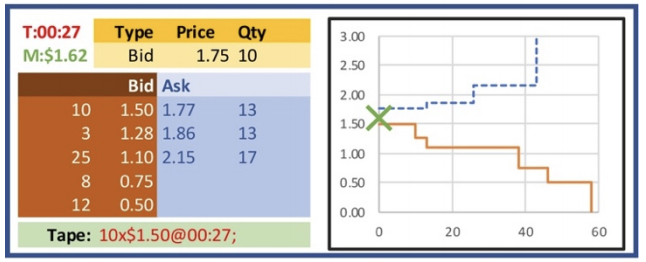
\includegraphics[width=0.8\textwidth]{LOB-Precross.png}
	\caption{A graphical representation of a Limit Order Book (LOB), reproduced from Cliff (2018)}
	\label{fig:Lob}  
\end{figure}
\noindent
The left hand side of Figure \ref{fig:Lob} is a mockup of a graphical representation of BSE, whilst in its original form, is in a python dictionary data structure.
As seen in the figure, the bid book lists all the bid orders with their prices and the respective quantities available at that price as a key/value pair in descending order to represent all the outstanding orders from the buyers. Conversely, the ask book lists the price-quantity pair for all the ask orders in ascending order. In this order, the highest bid price is at the top of the bid book alongside the lowest ask price: the two prices are called the \textit{best bid} and the \textit{best ask} respectively. 
\\
\\
This graphical representation allows for easy feature extraction for some key elements that may not explicitly stated in the figure. 
\begin{itemize}
\item The \textit{Time Stamp} for the current time in the trading session, shown post-facing the "T" in the top left corner
\item The \textit{Bid-Ask Spread} which is the difference between the \textit{best ask} and the \textit{best bid}
\item The \textit{Midprice} is the arithmetic mean of the \textit{best ask} and the \textit{best bid}
\item The \textit{Tape} shows a record of all the executed trades and cancellations of orders
\item The \textit{Microprice} is a cross volume weighted average of the \textit{best ask} and \textit{best bid}, prefaced by the green "M" below the time stamp
\item The latest limit order sent to the exchange by a trader

\end{itemize}
\noindent
The \textit{midprice} and \textit{microprice} are values that are used to approximate the value of the asset and attempt to summarise the market. In this example snapshot figure \ref{fig:lob} the \textit{best ask} is \$1.77 and the \textit{best bid} is \$1.50 so the midprice is (\$1.77 +  \$1.50)/2 = \$1.66. The \textit{microprice} is a more intricate calculation because it is a cross volume weighted average:


\begin{equation}
\label{microprice}
\begin{split}
\frac{BestBidQty * BestAskPrice + BestAskQty*BestBidPrice}{ BestBidQty + BestAskQty}  = Microprice 
\end{split}
\end{equation}
\begin{equation}
\begin{split}
\frac{5*\$1.77 + 13*\$1.50}{5 + 18} = \$1.58
\end{split}
\end{equation}

\noindent
The right hand side of Figure \ref{fig:Lob} represent the supply and demand curves calculated from the ask and bid books respectively, where the orange line is the demand curve and the blue line is the supply curve.  Following the orange or blue step functions from left to right, at each step, the height represents the price and the width represents the available quantity at the price point. Lastly, the green cross represents the microprice.
\\
\\
A trade occurs when a bid order price is greater than the \textit{best ask} or when an ask order price is less than the \textit{best bid} on the LOB, this is known as \textit{crossing the spread}. This process is quantity invariant, that is if the latest order price crosses the spread but the requested quantity exceeds the quantity available at that price, all the quantities that are available are sold crossed price, and the unfulfilled quantities are then placed on the LOB as an outstanding order.
\\
\\
\noindent
As seen in Figure \ref{fig:Lob}, the supply and demand curves do not cross, which therefore represents the fact that no trader is willing to trade at the current prices given in the exchange. The supply and demand curves not crossing means that the LOB is currently at equilibrium, as the best bid is not greater than the best ask.

\begin{figure}[H]
	\centering
	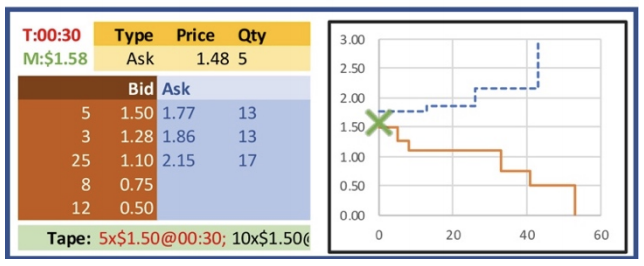
\includegraphics[width=0.8\textwidth]{LOB-Postcross.png}
	\caption{A graphical representation of a Limit Order Book (LOB), reproduced from Cliff (2018)}
	\label{fig:LobPost}  
\end{figure}
\noindent
Figure \ref{fig:LobPost} indicates that a new order has been placed to the exchange. Interestingly, this order crosses the spread because the ask price \$1.48 was less than the \textit{best bid} in Figure \ref{fig:lob} so therefore a transaction occurs. Incidentally, the quantity requested was less than the quantity available at \$1.50 so the entire order is fulfilled, and the quantity remaining is updated from 10 to 5. For arguments sake, if the quantity requested was 20 rather than 5, all the quantities that are available at \$1.50 (10) would be used to fulfil the new order and then the LOB would have a new \textit{best bid} of \$1.48 with a qty of 10. 
\vspace{1cm}
\subsection{Proprietary trader's Objective}
\vspace{0.5cm}
The agents that are taking part in the \enquote*{gamification} of the trading session are sales traders. The aim of the sales trader is to maximise their consumer surplus relative to their client's order. As mentioned in the previous chapter, the sales trader does not hold a stock of their own, they trade on behalf of their \textit{client}, who provides them with a limit price that they cannot buy or sell above or below respectively. The goal of the sales trader is to maximise the difference between the limit price and the trade price, which is the consumer surplus. In the real world, the sales trader makes commission based on the consumer surplus and the client pockets the rest. 
\\
\\
The proprietary trader's objective is that to maximise their own capital by buying and selling stocks for themselves. Whilst initially it may seem like the objective of the prop trader is different to the sales trader and therefore can't be compared, but the proprietary trader's ability to maximise the difference between the price they buy and sell a stock at is analogous to a sales trader maximising the difference between its limit price and its trade price. This rephrasing of the problem allows this project to directly compare the traditional machine learning approaches to the prop trader developed in this project.

\section{Traditional Sales Trader Solutions}
Chapter \ref{chap:context} outlined a brief history of various automated trading systems that contributed to the evolution of this field. It is important to gain a deeper understanding of the implementations of some of those trading systems as they serve as the foundations from which this project is built upon, and they are systems that are extensively used to evaluate how effective the system developed in this project is. 
\\
\\
\textbf{Zero Intelligence - Unconstrained (ZI-U) - Gode \& Sunder 1993}
\\
\\
\noindent
In 1993 Gode \& Sunder introduced a series of \textit{zero-intelligence} algorithmic traders designed for CDA markets. These were trading systems with very low level of intelligence that were placed into CDA markets to observe experimental trading markets where humans did very well in terms of allocative efficiency. The first of which is called Zero-Intelligence - Unconstrained (ZI-U). This is a trader that is not constrained in terms of a budget, it quotes a price selected from a uniform random distribution between the minimum market price and the maximum market price, irrespective of the client's limit price. Unsurprisingly, the ZI-U trader was not an effective solution to tackle the sales trader problem. 
\\
\\
\textbf{Zero Intelligence - Contstrained (ZI-C) - Gode \& Sunder 1993}\\
\\
Gode \& Sunder proposed another algorithm called Zero-Intelligence - Constrained (ZI-C). ZI-C is similar to ZI-U in that it quotes a price from a uniform random distribution, however, instead of the distribution ranging from the market maximum and market minimum price, the distribution ranges from the client's limit price to the maximum/minimum market price if the trader is a seller/buyer respectively. ZI-C is surprisingly human-like in many market conditions as alluded to in \ref{chap:context}, however is easily beaten by more sophisticated algorithms. 
\\
\\
\textbf{Zero Intelligence Plus - Cliff 1997}
\\
\\
Alongside Cliff's 1997 critique of Gode \& Sunder's 1993 paper, he developed the Zero Intelligence Plus algorithmic trader. This trader has a \enquote*{profit margin} which gets adjusted according to a learning rule. To elaborate, the price \textit{P}, at which the that the trader submits a buy/ask order, is a product of the limit price L plus some margin M: $L(1.0 + M)$. 
\\
\\
\noindent
It is important to make the distinction that the ZIP trader is \textit{adaptive} unliked ZI-U and ZI-C. The margin $M$ is constantly adjusted depending on the behaviour of the other traders in the market. If the ZIP trader is a seller, and the other sellers are accepting bids \textit{below} $P$, the ZIP trader decreases its margin (however constrained to be \textgreater 0). If the other sellers are accepting bids \textit{above} $P$, then the ZIP trader increases its margin. The buyers behave inversely to this. The rule that dictates how to adjust M is the Widrow-Hoff learning rule.
\\
\\
Cliff demonstrated that ZIP traders succeed in market conditions where ZI-C had failed, and demonstrated that they behave human-like in these markets.   
\\
\\
As mentioned in Subsection \ref{subsection:Experimental Economics to Algorithmic Trading} IBM demonstrated that ZIP outperformed their human counterparts in controlled experiments. So this project uses ZIP as the benchmark to explore if a DRL trader can be implemented that will too, outperform its human counterparts.  

\section{Reinforcement Learning}

This project transforms the current Prop trader problem to a problem that is well suited to a DRL paradigm, which will be the main avenue of solutions this project explores, so it is paramount to provide the technical background for reinforcement learning, which is the basis of this project.
\subsection{What is Reinforcement Learning}
Reinforcement Learning is the training of machine learning models(agents) to take actions that interact with a complex, to maximise a reward {\color{red}{ \cite{hey}}}. More formally, the agent learns, via interactions with an environment, a policy $\pi(\alpha|\sigma)$ which is the probability to take a particular action $\alpha$, after observing a state $\sigma$ that maximises its reward. 
{\color{red}{state all the sources for the derivations in the entire chapter}}
\\
\\
\noindent
\textbf{Markov Decision Process}
\\
\\
Most Reinforcement Learning requires a fully observable environment in which Markov Decision Processes (MDP) are a formalisation of this environment and the problem definition as a whole, where almost all RL problems can be formalised as. 
\\
\\
\noindent 
A MDP is a 5-tuple which has components that are defined as follows:
\begin{itemize}
\item $\Sigma$: The set of all states, where a state $\sigma_t$ is defined as an observation from an 
environment at time stamp t
\item  A: The set of all actions possible, where an action $\alpha$ is any action available to the the agent in state $\sigma_t$ at time stamp t
\item $\Phi$: The set of all transition probabilities, where $\phi_{\alpha_t}$ is the probability that action $\alpha_t$ in state $\sigma_t$ at time stamp $t$ will lead to state $\sigma'$ in time stamp $t+1$. 
$\Phi(\sigma_t, \sigma') = Pr(\sigma(t+1) = \sigma' | \sigma_t, \alpha_t)$. This is a stochastic process because the same state-action transition may not lead to the same state', which may due to random factors in the environment or interactions with the other agents, or an inaccurate interpretation of the current state from the agent, which is suitable for this project's environment. 
\item $\rho_{\alpha_t}(\sigma_t)$: The immediate reward after the transition from state $\sigma_t$ to an arbitrary state $\sigma'$ 
\item $\gamma \in [0,1]$: This is a discount factor representing the difference in importance between present and future rewards. Depending on the value of $\gamma$, it will encode the idea that a reward that is received in the present is more desirable/valuable than the same reward received at any point in the future. 



\end{itemize}
\vspace{0.5cm}
\noindent
Making MDP a 5-tuple:{$(\Sigma,A, \Phi, \rho,\gamma)$
\\
\\

\noindent
The goal of a MDP is to optimise a policy $\pi(\alpha | \sigma)$, which defines the probability that the agent should take an action $\alpha$ given an observed state $\sigma$, maximising a cumulative reward function of random rewards, i.e the expected discounted sum of rewards over an infinite time horizon. So, an agent during every time step in its existence, tries to maximise the expected return:

\begin{equation}
\label{discount-rewards}
\begin{split}
U(t) = \sum\limits^{\infty}_{t=0}{\gamma^{t} \rho(\sigma_t)}
\end{split}
\end{equation}

\vspace{0.5cm}
\noindent
Equation \ref{discount-rewards} establishes a measure of value for a given \textit{sequence of states}, however, this measure needs to be used to define the value for a \textit{specific state}. This measure ideally represents both the immediate reward, and a measure of of the agent \enquote*{heading in the right direction}, which in this context means to make a profitable trade, to accumulate future rewards.
\\
\\
To summarise so far, the \textit{utility} of a state is the expected reward received in the current state, plus the rewards we accumulate on the journey through future states, following a given policy. This definition is framed as an \textit{expectation} because the environment that is specified in this domain is stochastic, so future states are not deterministic. This notion of \textit{utility} is encapsulated in what is called the value function. 

\begin{equation}
\label{expected-discounted-rewards}
\begin{split}
V_\pi (\sigma) = E_\pi [U(t) | \sigma_t = \sigma]
\end{split}
\end{equation}

\noindent 
This equation can be rearranged with the derivation\cite{rearrange-value-function https://www.jeremyjordan.me/markov-decision-process/} to give:

\begin{equation}
\label{expected-discounted-rewards-rephrased}
\begin{split}
V_\pi (\sigma) = E_\pi [\rho(\sigma_t) + \gamma(V( \sigma_{t+1})) | \sigma_t = \sigma ]
\end{split}
\end{equation}

\noindent 
This now defines a function for calculating the utility of a \textit{specific state} as input, and the function returns a value for entering the given state.
\\
\\
Alongside this, the Action-Value function, an estimate of the value given an action is as follows:


\begin{equation}
\label{action-value}
\begin{split}
Q_\pi(\sigma , \alpha) = E_\pi [U(t) | \sigma_t = \sigma, A_t, = \alpha]
\end{split}
\end{equation}


\noindent 
Considering the fact that the agent is interested in the optimal policy, and the optimal policy is the sequence of actions, that maximise the utility until the \enquote*{game} is finished, the value function alone cannot be used, as it only provides the expected return from a specific state, but information regarding which action to take is not provided. If the value function is to be used alone, the agent would have to simulate all possible actions to determine which action takes the agent to the state with the highest utility, which impossible in this problem domain. The Action-Value function connects the expected returns with actions, which provides the agent with information on what action to take to maximise its utility. 
\\
\\
The derivation in \cite{rearrange-value-function https://www.jeremyjordan.me/markov-decision-process} allows the Equation \ref{expected-discounted-rewards-rephrased} to be rearranged in such a way that matches the format of a Bellman equation, which then allows the action-value Equation \ref{action-value} to be rearranged as a Bellman Expectation Equation, subject to a policy $\pi$:
{\color{red}{explain what a bellman equation is}}

\begin{equation}
\label{bellman}
\begin{split}
V_\pi(s) = E_\pi[R_t + \gamma V_\pi(S_{t+1} | S_t = s]
\end{split}
\end{equation}

\noindent
Which allows the Value Equation \ref{expected-discounted-rewards-rephrased}, in finite terms, to be expressed as:

\begin{equation}
\label{value-function-bellman}
\begin{split}
V_\pi(s) = \sum\limits^{}_{\alpha \in A}{\pi(\alpha | \sigma)} \sum\limits^{}_{\sigma'}{\sum\limits^{}_{r}{p(\sigma' , r | \sigma, a) \{r + \gamma V_\pi(\sigma')\}}}
\end{split}
\end{equation}

\noindent
As well as the Action-Value function Equation \ref{action-value}, expressed as:

\begin{equation}
\label{action-value-bellman}
\begin{split}
Q_\pi(s) = \sum\limits^{}_{\alpha \in A}{\pi(\alpha | \sigma)} \sum\limits^{}_{\sigma'}{\sum\limits^{}_{r}{p(\sigma' , r | \sigma, a) \{r + \gamma Q_\pi(\sigma')\}}}
\end{split}
\end{equation}
\vspace{0.5cm}

\subsection{Optimality}
\label{Optimality}

In an ideal scenario, the agent wants to find the optimal solution to the MDP problem. So, the definition of \enquote*{optimal} is as follows:

\paragraph{Optimal Value Function.} The optimal state-value function $V_*(\sigma)$ is the maximum value function over all policies: $V_*(\sigma) = \max\limits_\pi V_\pi(\sigma)$. In essence, there are all kinds of policies that the agent can follow in the Markov chain, but this means that the agent wants to traverse the problem in such a way to maximise the expectation of rewards from the system. 
 
\paragraph{Optimal Action-Value Function.} The optimal state-value function $Q_*(\sigma)$ is the maximum action-value function over all policies $Q_*(\sigma) = \max\limits_\pi Q_\pi(\sigma)$. This means that if the agent commits to a particular action, this provides the maximum possible returns out of every possible traversal thereafter. Crucially, if the agent knows $Q_*(\sigma)$, then it has found the best possible traversal, so it has \enquote*{solved} the entire problem. So informally, an MDP is solved if  $Q_*(\sigma)$ is solved.

\paragraph{Optimal Policy.} The optimal policy, is to best possible way for an agent to behave in an MDP. The previous two definitions define \textit{what} the reward is, but this defines \textit{how} to achieve the reward. To define what makes one policy better than another, a partial ordering is created over policy space. $\pi \geq \pi'  if  V_\pi(\sigma) \geq V_{\pi'}(\sigma), \forall \sigma$. 

The theorem \cite{MDP-theorem RL Course by David Silver - Lecture 2: Markov Decision Process} summarises that the optimal policy achieves the optimal value function as well as the optimal state-value function. 

\subsection{Challenges to Find Optimal Solutions}
The Bellman Optimality Equation is typically used to solve for trivial MDP problems however there are key challenges that are prevent it to be a solution in practice. 

\begin{itemize}
\item Bellman Optimality Equation is non-linear - as the Expectations are intractable 
\item No closed form solution ( in general)
\end{itemize}

\noindent
To deal with this challenges, there are very clever solutions that will be covered in the next section.

\section{Solving Reinforcement Learning}
\label{section:Solving Reinforcment Learning}
\textbf{Model-Free}
\\
\\
There are numerous methods designed, developed and tested to solve the MDP problem, such as dynamic programming. However, solutions that are similar in nature require a well defined model and environment. In most practices, the MDP agent does not know the environment and its intricacies, which must be figured out by the agent itself. \textit{Model-Free} solutions give up the assumption that the model is well defined for the agent, which is more ideal in practice.
\\
\\
\textbf{Model Free Prediction} 
\\
\\
This is an \enquote*{evaluation} task, where given a policy $\pi$ the agent evaluates its Value function $V_\pi(\sigma)$ as mentioned in Equation \ref{value-function-bellman}, which can be done recursively through via the Bellman equation until convergence. 
\\
\\
\textbf{Model Free Control}
\\
\\
\noindent
Control is about the method used to improve on a policy $\pi$ to find the optimal policy $\pi_*$ as outlined in Subsection \ref{Optimality}. This is done via a method called \textit{Policy Iteration}, where unlike the prediction problem which iterates over the Value Function, \textit{Policy Iteration} iterates over the Action-Value function in Equation \ref{action-value-bellman}. This is done via iterating over every $Q_\pi(\sigma, \alpha)$ value and greedily taking the action with the maximum expected return. However, this solution in particular ignores the concept of \enquote*{delayed gratification} in which an individual state may not give the agent the maximum expected return, but the states following it yield greater reward, which would be ignored with this greedy solution. 
\\
\\
\noindent
In general, solving the Bellman Equation is to recursively solve for Equation \ref{value-function-bellman} and Equation \ref{action-value-bellman} which is very inefficient as mentioned below Equation \ref{action-value}, so other solutions are explained below. 

\subsection{Model Free Prediction: Monte Carlo }
\label{Monte Carlo Prediction}
The Monte Carlo (MC) method is one of the simpler and intuitive solutions to the reinforcement learning problems
\begin{itemize}
\item MC methods learn directly from experience
\item MC methods have no prior knowledge of MDP transitions 
\item Uses the simplest possible idea: Using sample means from episodic experience 
\end{itemize}

\noindent
\textbf{Goal: } Given a policy $\pi$, learn $V_\pi$ from episodes of experience: $\sigma_1, \alpha_1, r_1,..., \sigma_k$
Recall that the value function uses the expected return, however, Monte Carlo uses the empirical sample means as an approximation for the expected return:
\begin{equation}
\label{Monte Carlo Mean}
\begin{split}
V_\pi (\sigma) = E_\pi [U(t) | \sigma_t = \sigma] \approx \frac{1}{N} \sum\limits^{N}_{i=1}{U_{i,\sigma}}
\end{split}
\end{equation}
\noindent 

\subsection{Model Free Control: Monte Carlo}
To solve the control problem, a greedy policy function is used w.r.t to the current value function. 
\begin{equation}
\label{Monte Carlo Control}
\begin{split}
\pi_*(\sigma) = arg\max\limits^{}_{\alpha}{Q_\pi(\sigma,\alpha)}
\end{split}
\end{equation}

\noindent
The major problem with this approach in this project's problem domain is the fact that because the state space in BSG is very complex, and because the Monte Carlo solution requires a \enquote*{reset} back to a specific state ${\sigma_t}$ to effectively approximate the expected returns, the solution is not a good fit for the problem at hand. 

\subsection{Model Free: Temporal Difference Learning - TD(0)}
\label{TD learning}
Temporal Difference Learning (TDL) is an \textit{online}-policy method in which the agent learns by updating its prediction at every time step throughout an episode, this differs to the MC solution as MC relies on episodic experiences as a whole to learn, rather than learning during the actual episode.  
\\
\\
In mathematical notation, this means that the value function $V_\pi(\sigma)$ is updated toward the \textit{estimated} return $\rho(\sigma_t) + \gamma V_\pi (\sigma_t)$:
\begin{equation}
\label{TD error}
\begin{split}
V_\pi(\sigma) \leftarrow V_\pi(\sigma) + \beta(\rho(\sigma_t) + \gamma V_\pi (\sigma_t) - V_\pi(\sigma_{t+1}))
\end{split}
\end{equation}

Where the estimated return is analogous to the Bellman Equation \ref{value-function-bellman}, in which $\rho(\sigma_t)$ is the immediate reward and $\gamma V_\pi(\sigma_t)$ is the discounted future reward for the next step and where $\beta$ is the generalised \textit{learning rate}. We substitute this \textit{estimated} return (otherwise known as the \textit{TD Target}) in for the \textit{real} return unlike in MC methods, which results in the \textit{TD error} of:

\begin{equation}
\label{TD error}
\begin{split}
\delta_t = \rho(\sigma_t) + \gamma V_\pi (\sigma_t) - V_\pi(\sigma_{t+1})
\end{split}
\end{equation}
\noindent
Intuitively this differs with MC methods because, in an example where the agent was driving a car and \textbf{almost} crashes, but then drives off safely: the MC method would not update the value function in a negative sense because the end goal was not negative, whilst with TD learning, the \textit{online} learning policy allows the agent to update the value function for the previous time steps leading up to the incident to change future behaviour. This is desirable behaviour for the prop trader problem as it means that the agent could potentially learn the states that lead up to a a sudden drop or rise in price of a stock, which the trader could have bided or asked for, which may have led to a loss. Whilst in MC the trader would have had to commit the to a bad trade to have learnt from the experience. 
\\
\\

\noindent 
To solve the control problem for TD Learning, there are various options that can applied to this kind of learning that follows the \enquote*{Generalised Policy Iteration} structure, with the exploration vs exploitation problem trade-off being achieved with the $\epsilon-greedy$ method. They are: \textit{SARSA, SARSAmax, Q-Learning, Expected SARSA}. The following equations have been obtained from \cite{https://www.cellstrat.com/2020/04/27/temporal-difference-methods/} 
\\
\\
\textbf{SARSA}
\\
\\
This method uses every element of the quintuple of events $(S_t, A_t, R_{t+1}, S_{t+1}, A_{t+1})$, inspiring the name \enquote{SARSA}. 
\begin{equation}
\label{SARSA}
\begin{split}
Q(\sigma_t, \alpha_t) \leftarrow Q(\sigma_t, \alpha_t) + \alpha[\rho(\sigma_t) + \gamma Q(\sigma_{t+1}, \alpha_{t+1}) - Q(\sigma_t, \alpha_t)]
\end{split}
\end{equation}
\noindent
This is an \textit{on-policy} method which means that the agent will learn by using the experience sampled by the same policy. 
\\
\\
\noindent
\textbf{SARSAmax/Q-Learning}
\\
\\
This is a \textit{off-policy} TD algorithm. This means that the learned action-value function, Q, directly approximates $Q_*$, the optimal action-value function. This occurs independent of the policy that is being followed. 
\begin{equation}
\label{Q-learning}
\begin{split}
Q(\sigma_t, \alpha_t) \leftarrow Q(\sigma_t, \alpha_t) + \alpha[\rho(\sigma_t) + \gamma \max\limits^{}_{\alpha}Q(\sigma_{t+1}, A) - Q(\sigma_t, \alpha_t)]
\end{split}
\end{equation}

\noindent
\textbf{Expected SARSA}
\\
\\
This is an \textit{on-policy} TD control algorithm. It is similar to Q-learning, with a slight variance. Instead of the maximum over next state–action pairs,  the algorithm uses the expected value, taking into account how likely each action is under the policy being used. Given the next state, $\sigma_{t+1}$, this algorithm moves deterministically in the same direction as SARSA moves in expectation. 
\begin{equation}
\label{SARSA}
\begin{split}
Q(\sigma_t, \alpha_t) \leftarrow Q(\sigma_t, \alpha_t) + \alpha[\rho(\sigma_t) + \gamma E_\pi[Q(\sigma_{t+1}, \alpha_{t+1}) | \sigma_{t+1}] - Q(\sigma_t, \alpha_t)]
\end{split}
\end{equation}

\noindent
All three control solutions for TD learning follow the same \textit{Policy iteration} procedures as outlined earlier in this section. 

\subsection{Value Function Approximation}
\label{subsection:value-function-approx}
In an ideal scenario, the discussed methods so far (MC and TD) would work for all reinforcement learning problems, however there is a critical hurdle that these solutions to not account for in real world problems. The solutions discussed thus far solve the reinforcement learning problems using \textit{tabular methods} i.e treating $V_\pi(\sigma)$ and $Q_\pi(\sigma, \alpha)$ as dictionaries, which is simply not a feasible solution for problems with a large state space. As examples, Backgammon has $10^{20}$ states, and the game AlphaGo Zero solved, \enquote*{Go}, has $10^{70}$ states. Backgammon is considered a small game, which provides some added perspective as to the scale of problems that reinforcement learning can solve. 
\\
\\
\noindent
This problem is tackled using \textit{Value function approximation}:

\begin{equation}
\label{value-approx}
\begin{split}
\hat{V}(\sigma, \textbf{w}) \approx V_\pi(\sigma)
\end{split}
\end{equation}

\begin{equation}
\label{action-value-approx}
\begin{split}
\hat{Q}(\sigma,\alpha, \textbf{w}) \approx Q_\pi(\sigma, \textbf{w})
\end{split}
\end{equation}
\noindent
These functions are parametric function \enquote*{approximators}, where \textbf{w} are the weights. So now, the parametric regression allows the approximator to generalise the previously denoted dictionaries as a general fitted function, which allows the agent to query the function for unseen/infinite state spaces. 


\begin{figure}[H]
  
	\centering
  	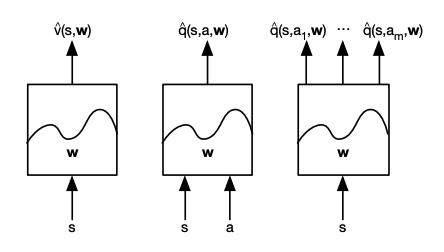
\includegraphics[width=0.8\textwidth]{value-approximators.png}
  	\caption{Types of value approximators, reproduced from Silver \cite{https://www.davidsilver.uk/wp-content/uploads/2020/03/FA.pdf}}
	 \label{fig:Approximators}

\end{figure}

\noindent
Figure \ref{fig:Approximators} shows the architectures of the varying types of approximators. The leftmost architecture represents a \textit{Value function} approximator, where a \enquote*{black-box} function spits out the \enquote*{value} of being in state \textit{s}. The middle architecture showcases the \textit{action-value} approximator, where again, a \enquote*{black box} function takes in the state the agent is in, and the action it is considering, and it spits out how good that action is. Lastly, the rightmost architecture represents an architecture that will give the agent the action-value for all possible actions in the given state \textit{s}. 
\\
\\
The natural step to take at this point is to choose the type of \enquote*{black-box}, and this project explores the usage of neural networks. Since neural networks are function approximators, they a play a crucial role in RL in scenarios where the state space or action spaces are too large to be completely known. They are used in the RL context to approximate the \textit{value function} or \textit{action-value functions} by optimising weights along gradients that promise less error. 
\\
\\
The methodology to optimise these weights is Stochastic Gradient Descent(SGD). To perform SGD a differentiable function is required with input parameter \textbf{w}, J(\textbf{w}) , where the gradient of J(\textbf{w}) is defined as:
\begin{equation}
\label{parameter-gradient}
\begin{split}
\nabla_\textbf{w} J(\textbf{w}) = \gradient
\end{split}
\end{equation}
In a supervised learning example, the goal is to find parameter vector \textbf{w} that minises the mean-squared error (MSE) between the approximated value function $\hat{V}(s, \textbf{w})$ and true value $V_\pi(\sigma)$ and then use SGD to find local minima as defined in \cite{https://www.davidsilver.uk/wp-content/uploads/2020/03/FA.pdf}:

\begin{equation}
\label{MSE-supervised}
\begin{split}
J(\textbf{w}) = E_\pi[(V_\pi(\sigma) - \hat{V(\sigma, \textbf{w}))^{2}}
\end{split}
\end{equation}
\noindent
However, considering the context is reinforcement learning, there is no objective truth for $V_\pi(\sigma)$, there are only rewards to indicate to the agent whether or not the actions are good or bad, which are acquired through experience. 
Luckily, the previous subsections covered precise this. The objective function can be defined with the help of the TD/MC method defined earlier as:
\begin{itemize}
\item For MC the \enquote*{objective truth} becomes the return $U_t$: $\Delta \textbf{w} = \beta(U_t - \hat{V}(\sigma_t, \textbf{w})) \nabla_\textbf{w} \hat{V}(\sigma_t, \textbf{w}$
\item For TD the \enquote*{objective truth} becomes the TD target $U_t$: $\Delta \textbf{w} = \beta(\rho(\sigma_{t+1}) + \gamma\hat{V}(\sigma_{t+1}, \textbf{w}) - \hat{V}(\sigma_t, \textbf{w})) \nabla_\textbf{w} \hat{V}(\sigma_t, \textbf{w})$
\end{itemize}

\subsection{Policy Gradient}
\label{subsection:Policy Gradient}
The last subsection explained the use of value approximation functions in Equations \ref{value-approx} and \ref{action-value-approx}, to pick actions greedily with $\epsilon-greedy$ methods to acquire the max $Q_\pi$ during policy evaluation - summed up as policy iteration. 
\\
\\
A more natural and direct approach may be to directly parameterise the \textit{policy} rather than the value functions - This is known as Policy-Based Reinforcement Learning. So now the policy will be manipulated directly, by controlling and learning the parameters to affect the distribution by which actions are picked: so the policy can be directly modelled as:

\begin{equation}
\label{Policy Gradient}
\begin{split}
\pi_\theta(\sigma, \alpha) = P[\alpha | \sigma, \theta]
\end{split}
\end{equation}
\noindent
The goal for policy based reinforcement learning is that for a given policy $\pi_\theta(\sigma,\alpha)$ with paramters $\theta$, find the best set of paramteres $\theta$. However, the notion of \enquote*{best} is ambiguous, and  which is why an objective function needs to be defined. There are numerous kinds of functions depending on the type of environment, however, considering that a market session is an episodic environment, which has the notion of a \textit{start-state}, the most suitable objective function is as follows: 
\begin{equation}
\label{Policy Gradient}
\begin{split}
J_1(\theta) = V^{\pi_\theta}(\sigma_1) = E_{\pi_\theta} [v_1]
\end{split}
\end{equation}
\noindent
This objective function encodes the notion that if the agent always starts in some start state $\sigma_1$ or if the agent has a distribution over $\sigma_1$, how does the agent maximise the total end reward.
\\
\\
To find the $\theta$ that maximises the objective function $J(\theta)$ to find the optimal policy $\pi_*$, the project considers gradient \textit{ascent}. 
\\
\\
Policy gradient algorithms search for a local maximum for the objective function $J(\theta)$ by ascending the gradient of the policy, w.r.t to the parameters $\theta$ 

\begin{equation}
\label{Policy Gradient}
\begin{split}
\Delta \theta = \beta \nabla_\theta J(\theta)
\end{split}
\end{equation}
\noindent
where $\nabla_\theta J(\theta)$ is the \textbf{Policy Gradient} and $\beta$ is the learning rate 
\begin{equation}
\label{Policy Gradient}
\begin{split}
\nabla_\theta J(\theta) = \policygradient
\end{split}
\end{equation}
\noindent
\textbf{Monte Carlo Policy Gradient}
\\
\\
To compute the policy gradient analytically by exploiting the likelihood ratio trick:
\begin{equation}
\begin{split}
\nabla_\theta \pi_\theta(\sigma, \alpha) = \pi_\theta(\sigma,\alpha) \frac{\nabla_\theta \pi_\theta(\sigma,\alpha}{\pi_\theta (\sigma, \alpha)} \\
= \pi_\theta(\sigma,\alpha) \nabla_\theta \log_{\pi_\theta} (\sigma,\alpha) 
\end{split}
\end{equation}
Which allows the equation to represent a familiar term in statistics and machine learning, the score function \cite{score-function} which allows the gradient ascent to maximise the log likelihood to tell it how to adjust the gradients.
\\
\\ 
For \textbf{discrete} actions, a \textit{Softmax} Policy is used, where the actions are weighted using a linear combination of features $\phi(\sigma,\alpha)^{T}\theta$, and then to convert this linear combination to a probability function, these are exponentiated:
\begin{equation}
\label{Policy Gradient}
\begin{split}
\pi_\theta(\sigma, \alpha) \propto e^{\phi(\sigma,\alpha)^{T}\theta}
\end{split}
\end{equation}

\noindent
To make the score function:
\begin{equation}
\label{Policy Gradient}
\begin{split}
 \nabla_\theta \log_{\pi_\theta} (\sigma,\alpha)  = \phi(\sigma,\alpha) - E_{\pi_\theta}[\phi(\sigma, \cdot)]
\end{split}
\end{equation}
Intuitively this means that the feature for the action that the agent actually took, minus the average feature for all the actions the agent might have taken. So, the score function summarises how much more of the given feature it has more than usual, and if it gets a more reward, then adjust the policy to do it more. 
\\
\\

\noindent
\textbf{Actor Critic Policy Gradient}
\\
\\
\noindent 
An alternative method is also explored in this project. In the MC Policy Gradient method, the notion of the action-value functions defined earlier in this chapter are completely ignored, and focuses on the policy itself. In addition, the MC policy gradient method also has a high amount of variance.  Contrastingly, the Actor-Critic method reintroduced the notion of the action-value function via value function approximation outline in subsection \ref{subsection:value-function-approx}, whilst also aiming to reduce the variance.

The main component in this method is that a \textit{Critic} is used to explicitly estimate the action-value function, rather than using the returns of the episode experience.
\begin{equation}
\begin{split}
Q_w(\sigma,\alpha) \approx Q^{\pi_{\theta}} (\sigma, \alpha)
\end{split}
\end{equation}

The Actor-Critic algorithms maintain two sets of parameters:
\begin{itemize}
\item Critic - Updates the action-value function paramters: w
\item Actor - Updates policy parameters $\theta$, in the direction suggested by the critic
\end{itemize}

\noindent
The actor is the entity that actually makes the decision in the environment. The critic merely observes the actor, however, it evaluates the actor's decisions. 
The critic element is introduced in order to reduce the high variance experienced from using MC Policy Gradient methods.This methodology is unique in the sense that it combines the previously explained Value-based methods, as well as the newly defined Policy-based methods.  Unsurprisingly, this method follows the overarching structure of policy gradient methods, however, they are defined as an \textit{approximate} policy gradient:
\begin{equation}
\begin{split}
\nabla_\theta J(\theta) \approx E_{\pi_{\theta}} [\nabla_\theta log_{\pi_{\theta}}(\sigma,\alpha) Q_w(\sigma, \alpha)]\\
\Delta \theta = \beta \nabla_\theta log_{\pi_{\theta}}(\sigma,\alpha) Q_w(\sigma, \alpha)
\end{split}
\end{equation}

\noindent
The main idea here is that the actor adjusts the policy parameters in the direction that, according to the critic, will get more reward. So, the true action-value function is replaced by the critic's approximation of this function using a neural network. 
\\
\\
\noindent
The natural question is how the critic is estimating the action value function, luckily this was covered in subsections \ref{Monte Carlo Prediction} and \ref{TD learning}, because this is a policy evaluation problem. 

%
\subsection{Discrete vs Continuous Action Spaces}
\label{subsection:Discrete Vs Continuous Action Spaces}
The methodologies described in the latter part of the chapter are versatile because they support problem scenarios with have discrete and continuous action spaces. In the scenario where the action space is discrete, the solutions allow for a stochastic probability distribution between all the possible actions. E.g if there are five possible actions that the agent can take throughout the \enquote*{game}, the probability of these actions will change as the agent learns from experience, and these actions are sampled from the distribution. 
\\
\\
Methods which can optimise for continuous action spaces are applicable to many real world scenarios which make the the implementations of the policy gradient methods desirable. Now, instead of a distribution over a finite set of actions, the agent can now optimise for actions which involve real numbers.
\\
\\
\noindent
Both types of action spaces are applicable to solutions to solve the prop trader problem, and both are explored throughout the project.
%\subsection{DDPG}

\section{Summary}`
\noindent
This chapter aimed to summarise the difficult technical challenges of the prop trader problem as well as the plethora of techniques that are traditionally used to solve reinforcement problems. The chapter started with providing the necessary context to understand how reinforcement learning is structured as a problem, and then the consequent sections built up the necessary knowledge to understand the main solutions outlined in the latter sections of the chapter. The project will aim to implement these techniques. 

% -----------------------------------------------------------------------------

\chapter{Project Execution}
\label{chap:execution}
\vspace{1cm}

\noindent 
This chapter intends to describe the entire journey of project. From the birth of the idea of the project, to the implementation and critical analysis of results. 
{\color{red}{Talk about merging chapters 3 and 4 because the nature of project - intertwined}}
\\
\\
\section{Origin}
In a Bristol University Computer Science fourth year module called \textit{Internet Economics and Financial Technology} Prof Dave Cliff and Dr John Cartlidge conducted intriguing experiments which used students on the course to demonstrate that human traders in a continuous double auction gravitate to a market equilibrium price when trading under a time constraint. Furthermore, the course outlined outstanding algorithms (ZIP, MGD, AA), that were developed and outperformed their human counterparts in this very experiment - this is where the motivation and intrigue behind the project was born. 
\\
\\
\noindent
Considering the fact that these algorithms were sales traders who traded with a limit price given by their clients: what if there was an algorithm designed for a proprietary trader that similarly outperformed humans at this task?

\section{The Deeply Reinforced Trader}
As a reminder, RL, and by extension DRL, is a type of machine learning technique that allows an agent to learn in an interactive environment, via trial and error using feedback from its own actions and experiences. The overall process architecture of this kind of learning is as follows: 

\begin{figure}[H]
\centering{
  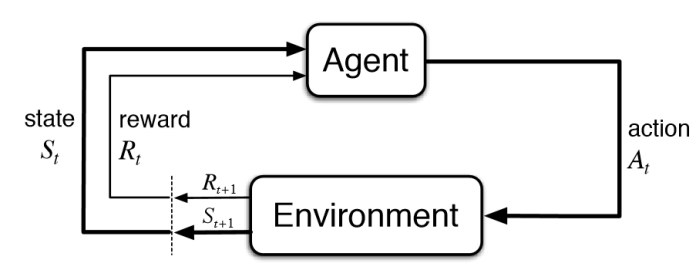
\includegraphics[width=0.8\textwidth]{RL-architecture.jpg}
  \caption{Architecture of Reinforcement Learning Environments}
  }
\label{fig:RL-arch}  
\end{figure}

\noindent
Where:
\begin{itemize}
\item Environment: is the world that the agent operates 
\item State $S_t$: The current obserevation of the environment
\item Reward $R_t$: The feedback from the environment
\item Policy: The method to map the state to the agent's action 
\item Action $A_t$: The agent's action after observing the state
\end{itemize}

\vspace{0.5cm}


\subsection{Training Environment}

\noindent
Considering this architecture and problem definition, this project required a framework that processes a trading environment in this exact manner. Luckily, Furlan-Falcao outlined a framework developed as part of the thesis - called Bristol-Stock-Gym (BSG). BSG is a simulated trading environment that is a refactor of Cliff's Bristol Stock Exchange (BSE) that provides a framework to train RL models in the context of BSE. This framework is analogous to the frameworks that \textit{OpenAI}'s Python library \textit{Gym} provides to train models in this manner. 
\\
\\
\begin{lstlisting}[label=main-loop, caption = Main loop to step through trading environment]
for i in range(Episodes):
        environment = Environment(traders_spec, order_sched,time_step = time_step, max_time = end_time, min_price = 1, max_price = end_time, replenish_orders = True)
        done = False
        observation = environment.reset()
        while not done:
            action = trader_strategy(state)
            observation_, reward, done, info, balance = environment.step(action)
            trader.store_rewards(reward)
            observation = observation_
\end{lstlisting}
\vspace{0.5cm}
\noindent
To elaborate on the implementation above, the environment is initialised via the following steps:  Initialising an empty \texttt{Exchange},populating the market with traders ( specified by a \texttt{traders\_spec} which defines what types of traders to populate the market with), resetting the market session time to \texttt{1} and getting the initial observation. During an \textit{epsiode}, the trader looks at the observation, takes an action and gives it to the environment to make one \textit{step}. One \textit{step} through an environment allows each trader in the market to react the the current market conditions by placing an order or by updating their internal variables. If a trade occurs, both parties are notified, and then this trade is published in the lob. This process is repeated till the max time \texttt{1000} is reached, which signifies the end of one \textit{Episode}. 
\\
\\
\noindent
This project utilises Furlan-Falcao's BSG heavily in this manner, whilst training several different types of agents with different \textit{Trading Strategies} shown in the code snippet above.

\subsection{Designing the State}

The state in an RL environment is an observation made by the agent which essentially is a snapshot at time \textit{t} of crucial details in the environment that are useful to the agent, so the design of this state is crucial to the success of the trader's interpretation of the current environment, to best inform its decisions to maximise its reward. 
\\
\\
\noindent
In BSG, the environment provides an observation which is as follows:


\begin{lstlisting}[label=BSG-Obs, caption = BSG Environment Observation: LOB]
def get_public_lob(self, time):
        public_data = {}
        public_data['time'] = time
        public_data['bids'] = self.bids.lob_anon
        public_data['asks'] = self.asks.lob_anon
        public_data['tape'] = self.tape
        return public_data
\end{lstlisting}
\noindent
The data provided by this observation, and their significance, are outlined in section \ref{Technical:LOB}. This observation includes the current \textit{Asks} and \textit{Bids} in the market, the current time, and the tape - which captures all the trades that have taken place and all the cancelled orders by the traders in the market.
\\
\\
The problem with this observation from the environment is that it is of a variable size. At time $t=1$ the \textit{tape} would be of length 0, similarly with the \textit{bids} and \textit{asks}, however given an arbitrary time $t = k$, the size of these data structures can vary quite heavily. The reason as to why this is a problem is that most Deep Learning model architectures require a fixed input size, so the default observation data provided is not appropriate to use. It is noteworthy, that ideally the entirety of this observation can be used as an effective input as it is the maximum amount of information the agent could use, however, in a practical sense, this is unmanageable as the data increases linearly with time, which would make the agents state space too large.
\\
\\
\textbf{Latent Representation: Auto Encoder}
\\
\\
Research indicates that the local spatial structure in limit order books are key components in predictive analysis about the future behaviour of markets \cite{Deep learning for limit order books paper in research folder}. The paper explores and demonstrates how data in a LOB beyond the best bid and the best ask (which are directly used to calculate the midprice and microprice) can be used to regress to future prices with significant accuracy. This is down to the lower levels of the LOB indicating the varying levels of aggressiveness in the traders since they are more prone to cancellations and updates. This  theory would be appropriate for a trader in BSG as it may be an excellent way to for the trader to predict buy and sell opportunities. Thus, the design of the state space has incorporated this ideology. 


\begin{figure}[H]
	\centering
  	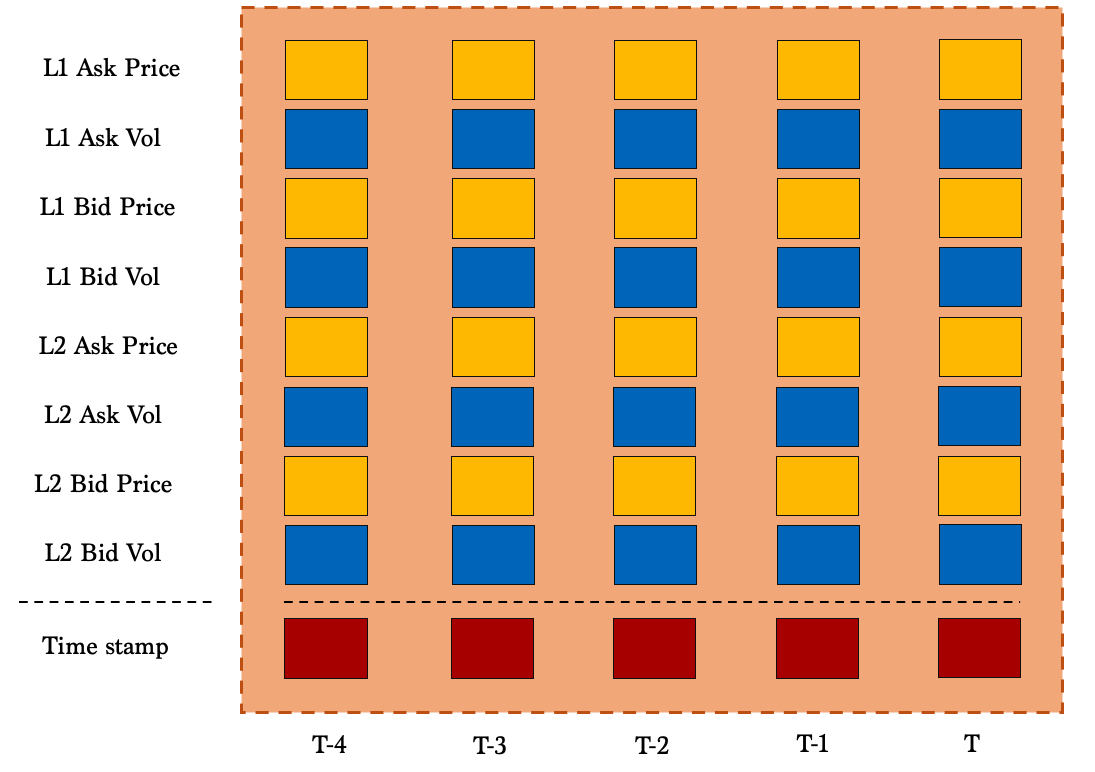
\includegraphics[width=0.5\textwidth]{LOB-Snapshot.png}
 	\caption{Capturing LOB Data}
	\label{fig:LOB-Snapshot}  
\end{figure}
\noindent
To capture trends in the LOB, the five latest changes to selected details in the LOB are stored as a matrix. The matrix is formed of five, \textit{1x9} vectors which contain the price and volume of level one and level two of the bids and asks and the current time stamp for the values that are currently on the LOB. It is important to note that the time steps are not necessarily consecutive in singular time steps, they are merely the time steps in which any change occurs to the non-time values in the LOB. 
\\
However, similarly to the case of using the entirety of the observation as the state space, this is a complex and high dimensional state space which will increase learning time significantly for the trader's models.  
\\
\\
To deal with this high dimensional state space, this state space heavily reduced via an Auto-Encoder (AE). 
\\
\\
An AE is a neural network (NN) that attempts to learn to copy its input to its output. It manages this task because of it is constituted by two main parts: an encoder that maps the given input to a smaller latent code, and a decoder that maps this latent code to a reconstruction of the original input. The role of the AE is to find an abstract and low-dimensional representation of the input to allow for easier learning and to compress and extract the crucial information out of an otherwise large state space. This is crucial in this problem scenario as the trends that would be apparent in the matrix outlined in Figure \ref{fig:LOB-Snapshot} would take significant time to learn with a matrix of size \textit{9x5}
\\
\\
\\
\\
\\
The architecture of the implemented AE is as follows:
\begin{figure}[H]
\centering{
  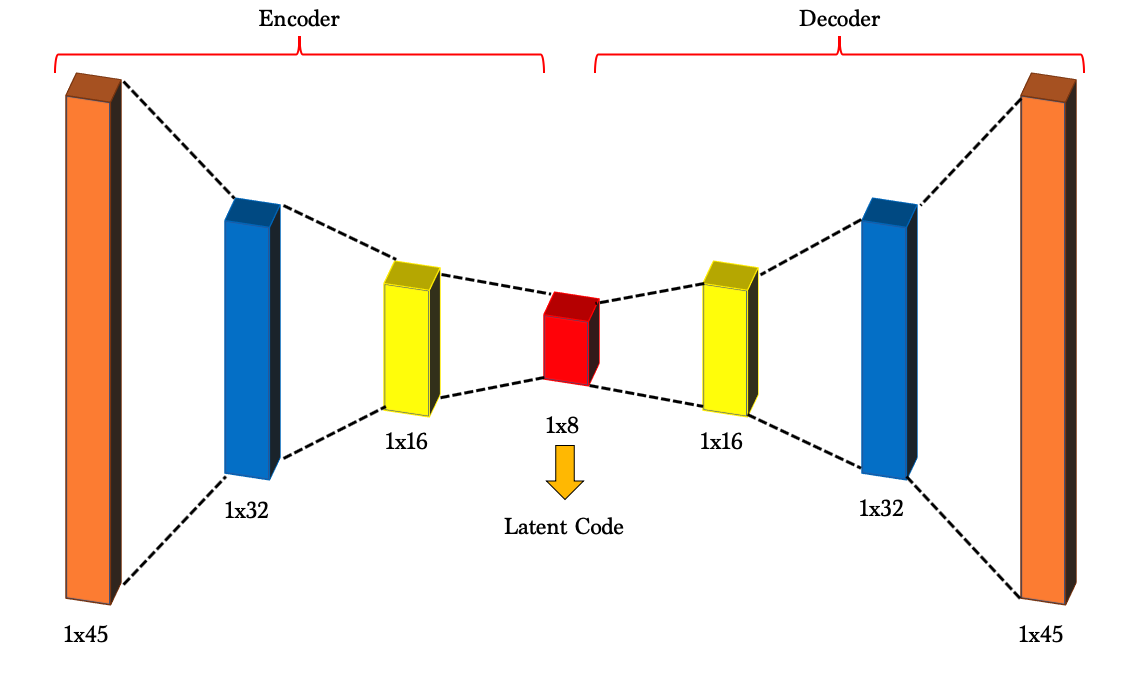
\includegraphics[width=0.8\textwidth]{AE-Architecture.png}
  \caption{Architecture of Auto-Encoder}
  }
\label{fig:AE-arch}  
\end{figure}
\noindent 
The \textit{5x9} input matrix is flattened to be an input into a \textit{linear layer} which is then compressed via a series of \textit{tanh} activation functions and linear layers - which were the constituents of the encoder. The compressed latent code is a vector of size \textit{1x8}, which is then decompressed via a series of \textit{tanh} activation functions and linear layers, into the AE model's approximation of the input - which made up the decoder. 
\\
\\
The model was trained on inputs collated from twenty market sessions which amounted to a dataset of size 1,032,290 of stacked \textit{5x9} matrices, which was split with a ratio of 7:3 to form the training and test data set respectively. The model was trained till convergence of test accuracy and saved for later usage. {\color{red}{specify accuracy + talk about how the error is minimised between the input and output of decoder}} 
\\
\\
The latent state representation was then concatenated to a vector consisting of the latest 8 trades that occurred in the market session. The design decision behind this is so that the trader can learn the relationships between the profitable trades that occurred in the market session and the other 8 features that were extracted from the AE. 
\\
\\
To incorporate more definitive features about the current state of the LOB, two more features were added to the state space. The first feature was the midprice of the market at the current time stamp $t$, this is to inform the trader as to what the best estimate of the price of the commodity is based on the orders placed on the LOB. The second additional feature was the current \textit{position} of the trader. The \textit{position} of the trader is encoded as a normalised value between -1 and 1. This value represents if the trader has an open position. To elaborate, if the trader has entered a trading position by having bought a commodity at price $x$, the current position is encoded as $[0.x]$ (the position would be encoded as $[-0.x]$ if the trader entered a trading position by selling a commodity at price $x$). The motivation behind adding these two values is for the trader to learn the connection between its current position and the appropriate action to take, for example if it has just bought a commodity, it now needs to sell it, and vice versa. 
\\
\\
The final form of the state space becoming a 18-tuple input vector as follows:
\begin{equation}
\label{Final state}
\begin{split}
[AE_1,AE_2,AE_3,AE_3,AE_4,AE_5, AE_6, AE_7, AE_8, \\Trade_1,Trade_2, Trade_3, Trade_4, Trade_5, Trade_6, Trade_7, Trade_8,\\ midprice_t, position_t]  
\end{split}
\end{equation}

\noindent
Where $AE_{1-8}$ are the data points provided by the latent state representation \textit{1x8} vector from the AE. 

%Papers have used 5 snapshots, to capture trends
%
%VAE to en
\subsection{Varying Supply and Demand Schedules}
\subsection{Discretised Strategy}
\label{subsection:Discretised Strategy}
As detailed in Subsection \ref{subsection:Discrete Vs Continuous Action Spaces} this context allows varying implementations of DRL techniques that utilise discrete and continuous action spaces. The actions discrete and continuous action spaces can be manipulated in the design of a \texttt{Trader\_strategy} function, which will convert the output of a neural network into an action compatible with BSG. 
\\
\\
The first approach taken was to discretise the action space to reduce the entire trading process of the agent down to a selection of three actions based on the observed state space.
\\
\\
The actions are as follows: 
\begin{itemize}
\item Action 0: NULL 
\item Action 1: Place a bid order
\item Action 2: Place an ask order
\end{itemize}

\noindent
The missing information from this strategy is that the price at which the trader submits a bid or ask order is so far undefined. To solve this issue, if the trader decides to place a bid/ask order (via Actions 1/2 respectively), the current $midprice_t$ (midprice at time stamp $t$) of the commodity is used as the price of the order. It is important to note that if the agent decides to place a buy order at price: $midprice_t$, the order may not necessarily lead to a transaction, it will have to be processed by the exchange. 
\\
\\
Initially, Action 0 may seem useless, however it is a crucial action as it will allow the trader to wait for the perfect circumstances to submit orders to the LOB and can allow the the trader to wait for the prices on the LOB to favour a profitable trading scenario.
\\
\\
This turns the problem into a classification task, as the agent would ideally learn what state correlates to a buy/sell opportunity effectively to perform profitable trades. 

\subsection{Vanilla Reward}
\label{subsection:Vanilla Reward}
One of the most crucial aspects in DRL is to formulate an effective reward system that enables the trader to learn the desirable behaviour. This is not a trivial task as it is one of the central challenges described in Section \ref{section:Central Challenges}. A perfectly reasonable design in the reward system may not yield the expected behaviour from the trader, so it is important to find the optimal system that allows the trader to learn to behave appropriately. This is analogous to supervised learning in which a network is fed data alongside truth labels; in this context, the trader must learn these labels by itself with the help of a well tuned reward system. 
\\
\\
\noindent
The first reward system changed the reward $r$ as follows: 

\begin{equation}
\label{Vanilla Reward}
\begin{split}
R(t) = \Delta TradePrice_{t=time\_of\_ sell, t=time\_of\_buy}
\end{split}
\end{equation}

\noindent
This is simply the difference in the price at which the trader sold the commodity at and the price at which the trader bought the commodity at. 

\begin{itemize}
\item $R(t) = 0$ : This will be the most common reward acquired by the trader per time step, as it implies that the trader has not engaged in any trade. This may be down to the fact that the current bid/ask order has not crossed the spread as explained in Subsection \ref{subsection:The Limit Order Book} or that no order has been submitted by the trader. An edge case scenario of the trader receiving this reward is if a trade has taken place, but the trader has \enquote*{broke even} which means that the trader bought and sold the commodity at the same price, meaning no profit or loss.
\item $R(t) > 0$: This reward means that the trader has made a profitable trade. Ideally the trader constantly acquires this reward throughout a trading session. Trivially, a profitable trade is rewarded with positive reward, however, the vanilla reward is most basic form of reward as it is a \textit{1 to 1 mapping} between the profit acquired and the reward received. 
\item $R(t) < 0$: This reward indicates that the trader engaged in a trade that incurred a loss. Considering the ZI-C and ZIP algorithms have the hard coded constraint of not trading at a loss, this reward aims to replicate this behaviour by penalising bad trades.
\end{itemize}

\noindent
This is denoted as a \textit{Vanilla Reward System} as this is the simplest form of reward system for a trader, which is a good starting point. 

\subsection{The PG Vanilla Agent}
In Furlan-Falcao's thesis, a Policy Gradient (PG) agent was implemented which provided interesting results. However, the thesis' implementation of the PG Agent explored a continuous action space to train the model to price asset at every time step. This project's implementation of the PG agent will interact with the environment via the discrete action space as defined in Subsection \ref{subsection:Discretised Strategy}. This implementation is based on the Monte Carlo Policy Gradient explained in Section \ref{subsection:Policy Gradient}, which means that the agent learns after completing an entire \enquote*{episode} and using that experience to adjust the model parameters via gradient \textit{ascent}.
 
\noindent 
This model is denoted as \textit{PG Vanilla} as it incorporates the vanilla reward system. 
\subsection{Analysis and Evaluation of PG Vanilla}
\label{subsection:Analysis and Evaluation of PG Vanilla}
\begin{figure}[H]
	\centering
  	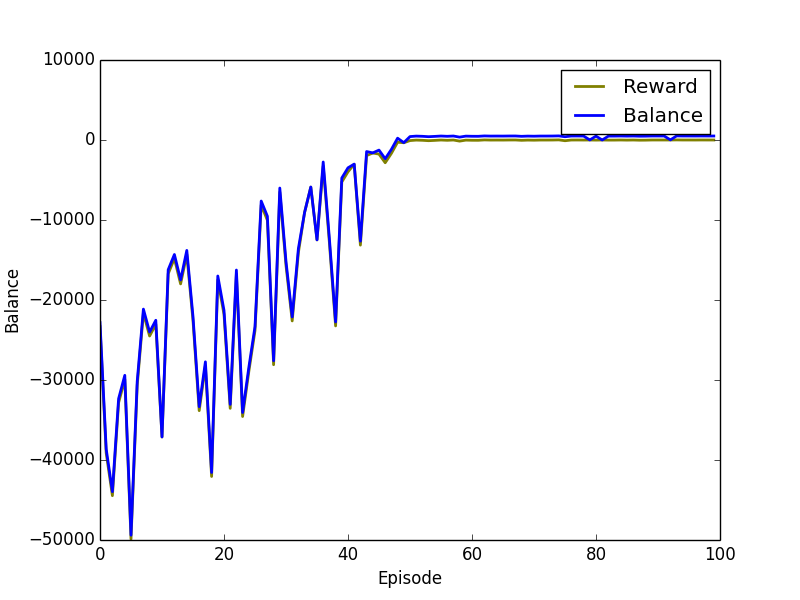
\includegraphics[width=0.8\textwidth]{PG-Vanilla-Reward.png}
  	\caption{Total reward over 100 iterations of the PG Agent in a market evenly populated with ZIC, ZIP and GVWY traders. }
	\label{fig:PG-Vanilla-Reward}  
\end{figure}

The graph appeared to indicate promising results as the trader's balance steadily increased from from a trough of approximately -£50,000 in episode five, where the trader constantly engaged in trades that result in a loss, to episode fifty-five which indicated that the trader breaks even. The plotted blue line represents the balance. This is parallel to the line that plots the reward, however there is a constant difference of £500, because that is the balance that the trader starts off with. 
\\
\\
However, upon inspection, the steady increase in balance was not down to the trader engaging in better trades, but down to the fact that the trader engaging in less trades. 

\begin{figure}[H] 
	\centering
  	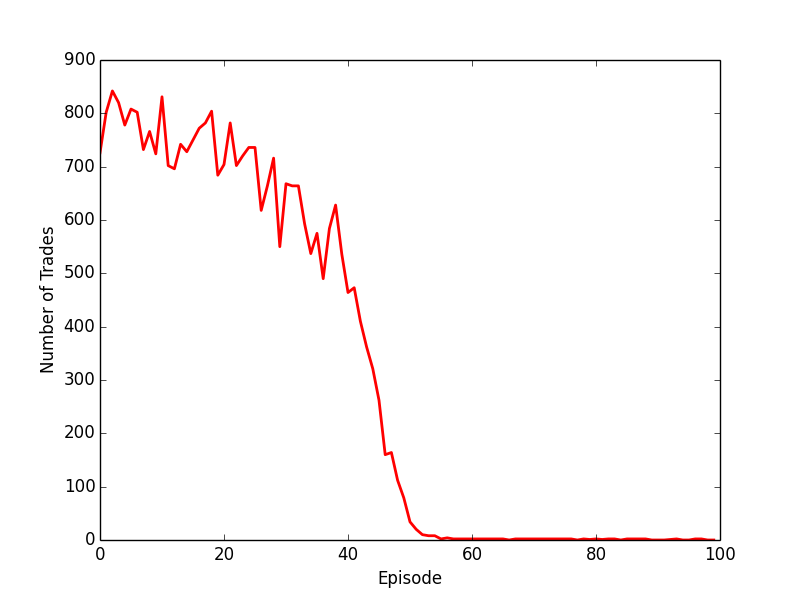
\includegraphics[width=0.8\textwidth]{PG-Vanilla-Num-Trades.png}
  	\caption{A plot of the number transactions the PG Vanilla agent engaged in during each episode }
	\label{fig:PG-Vanilla-Num-Trades}  
\end{figure}

\noindent
This was a hugely interesting result that was informative about the learnt behaviour of the trader. The trader began the learning process by exploring the action space randomly choosing discrete actions:Buy/Sell/NULL. This resulted in the trader engaging in a large number of trades, with a peak of 842 trades in episode two to a fast decline of an average of 0 trades after episode fifty. 
\\
\\
\noindent
To perform a more complete analysis of the results, it was crucial to figure out if the trader improved the rate at which it traded profitably, out of the trades that it was involved in. This was an important step because it provided an oversight as to whether the trader, in conjunction with learning to trade less, was learning to trade profitably too.

\begin{figure}[H] 
	\centering
  	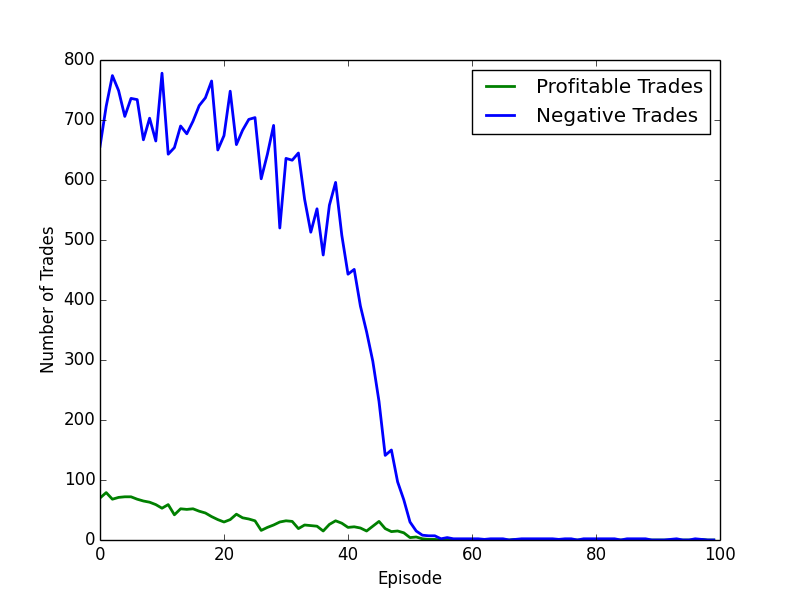
\includegraphics[width=0.8\textwidth]{PG-Vanilla-Good-Vs-Bad-Trades.png}
  	\caption{A plot of the number of profitable trades and trades that incur a loss for the trader }
	\label{fig:PG-Vanilla-Good-Vs-Bad}  
\end{figure}

\noindent
Figure \ref{fig:PG-Vanilla-Good-Vs-Bad} suggests that the trader did not improve in its ability to make a profitable trade. The hard coded property of ZI-C and ZIP traders to not trade at a loss was not learnt by the trader in its experience over 100 iterations. Therefore the rate at which the trader traded profitably did not increase relative to the number of trades. However, this result was interesting nonetheless. Since majority of the rewards received by the trader had been negative, it seemingly has learnt to increase its total reward by not trading at all. This is the exactly like the case of the Lunar landing analogy given in Section \ref{section:Central Challenges} in which the agent learnt to avoid a landing penalty by not landing at all. All in all, this is not desirable behaviour as the trader should ideally learn to trade \textit{profitably} and \textit{frequently}.
\\
\\
\noindent
It was important at this stage to evaluate and scrutinise the implementation to figure out which aspect of the MDP was causing this behaviour. The most obvious factor for the reasons behind this behaviour is the reward system. Expecting the system to learn what a good trade is via a simple \enquote*{Vanilla} profit and loss based reward system seemed be unrealistic - as it lacked guidance for the trader to incentivise it to take part in good trades. Other factors include: hyper-parameters of the models, the model architectures, and the state-space design. Ideally, all these factors would be explored to improve the model, however, given time constraints, the chosen reward system being rather simplistic and that reward systems play a crucial factor in the behaviour of a DRL-based trader, it was natural to explore this factor further with experimentation.

{\color{red}{Add the average loss per bad trade and average profit from good trades}}

\subsection{Optimising The Reward Function}
Whilst creating reward systems, the intended behaviour of the agent in training may not be realised, which Bonsai denotes as the \enquote*{cobra effect}\cite{https://medium.com/@BonsaiAI/deep-reinforcement-learning-models-tips-tricks-for-writing-reward-functions-a84fe525e8e0}. To elaborate, the article mentions that within the realm of RL, the agents behave as they are incentivised which may not align with the programmers intentions. 
\\
\\
After analysing the current reward system outlined in Subsection \ref{subsection:Vanilla Reward}, it became apparent that it does not guide the trader to learn what a good trade looks like before the eventual P\&L reward after buying and selling the commodity. In hindsight, considering that the trader constantly engaged in bad trades, it was no surprise that the trader stopped engaging in trade so that it minimises its loss rather than to maximise its gain. 
\\
\\
To tackle this issue, a new reward system was devised as follows:
\\
\\
For notation's sake, the Vanilla Reward System was renamed.
\begin{equation}
\label{Vanilla Reward}
\begin{split}
U(t) = \Delta TradePrice_{t=time\_of\_ sell, t=time\_of\_buy}
\end{split}
\end{equation}

The new reward $R(t)$ system became: 
\begin{enumerate}
\item R(t) = -10 : \texttt{if there is no order sent to the exchange}
\item R(t) = 10*U(t) : \texttt{if U(t) > 0}
\item R(t) = 2*U(t) : \texttt{if U(t) < 0}
\item R(t) = 10 :\texttt{if (Action == SELL and trader.position == BOUGHT and current\_midprice \textgreater  price bought )}
\item R(t) = 10 :\texttt{if (Action == BUY and trader.position == SOLD and current\_midprice \textless  price sold )}
\item R(t) = -10 :\texttt{if (Action == SELL and trader.position == BOUGHT and current\_midprice \textless  price bought )}
\item R(t) = -10 :\texttt{if (Action == BUY and trader.position == SOLD and current\_midprice \textgreater  price sold )}
\end{enumerate}
\noindent
The motivation behind a reward system of this kind was to provide more detail and guidance for the trader to learn what constitutes of making a good trade. 
\\
\\
Considering that the PG Vanilla agent eventually ceased to engage in any trading activity, reward 1. was devised to prevent the trader from remaining inactive in the trading session. This acts as a punishment for not submitting orders to the market. 
\\
\\
Reward 2. is designed to amplify the rewards of profitable trades. The motivation behind this was, considering the trader does not engage in many profitable trades relative to bad trades, to heavily reward the actions that lead to profitable trades. The same logic was applied to punishing the trader for bad trades , however a smaller multiplicative factor was used; this was done deliberately as the magnitude of the average loss for a bad trade was greater than the magnitude of the average profit for good trades as outlined in Subsection \ref{subsection:Analysis and Evaluation of PG Vanilla}, thus weighting positive rewards more than negative rewards.
\\
\\
 The last four features in the reward system make up the guidance element talked about previously. Since the trader's willingness in its actions to buy or sell may not necessarily translate into a trade, this reward system rewards the trader based on its intention/action, regardless of whether a transaction had taken place. If an order, comprised of the current midprice and a bid/ask type, is sent to the exchange that favours the trader to make a profitable trade, it is rewarded. Conversely, it is punished if the action chosen leads to an order submitted to the exchange which would lead to a loss. This idea to reward the \textit{intention} of the trader in conjunction with the P\&L was chosen to increase the probability in the trader engaging in better quality trades and to learn the hard coded constraints in the ZI-C and ZIP algorithms of not trading at a loss.  
\\
\\
The results of training the model using this reward system was as follows {\color{red}{get data for this}}: 

\subsection{Analysis of Optimised Reward System}
\label{subsection:Analysis and Evaluation of PG Vanilla}
\begin{figure}[H]
	\centering
  	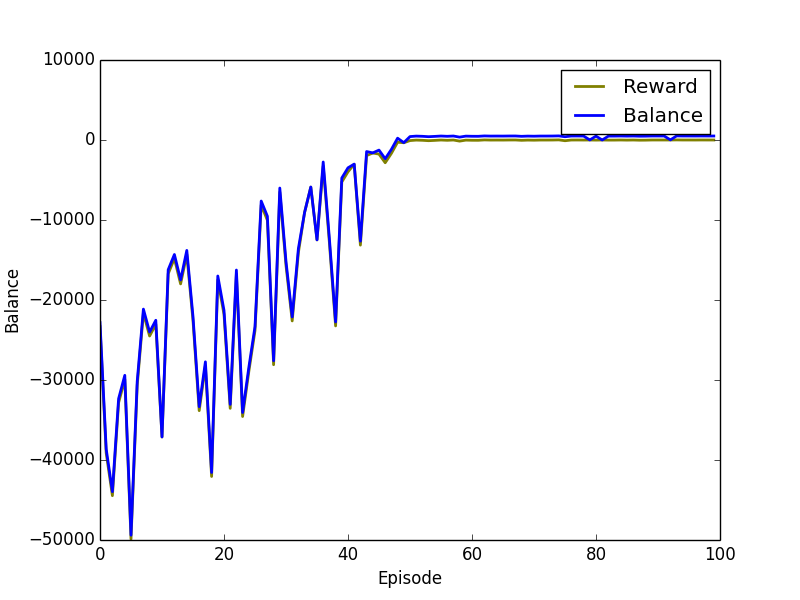
\includegraphics[width=0.8\textwidth]{PG-Vanilla-Reward.png}
  	\caption{Total reward over 100 iterations of the PG Agent with an optimised reward system }
	\label{fig:PG-Optimised-Balance}  
\end{figure}




\begin{figure}[H] 
	\centering
  	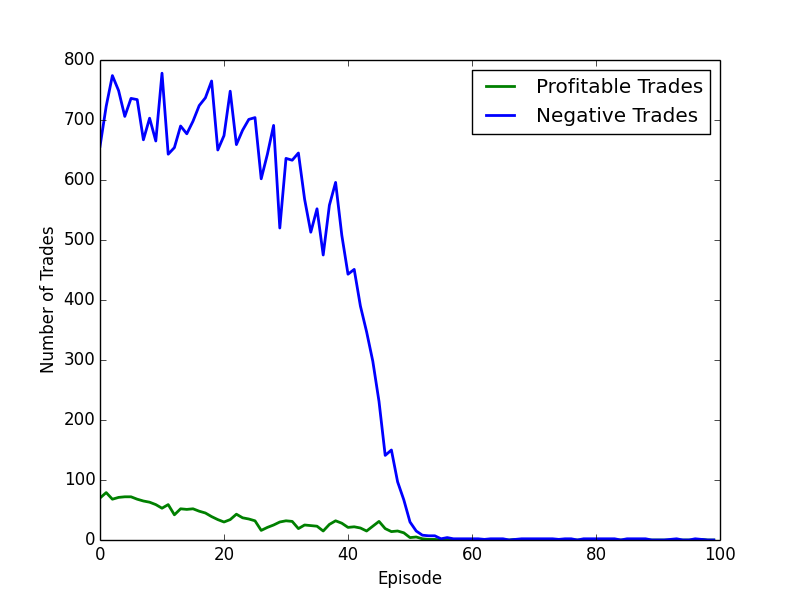
\includegraphics[width=0.8\textwidth]{PG-Vanilla-Good-Vs-Bad-Trades.png}
  	\caption{A plot of the number of profitable trades and trades that incur a loss for PG-Optimised }
	\label{fig:PG-Optimised-Good-Vs-Bad}  
\end{figure}

As seen in Figure \ref{fig:PG-Optimised-Balance}, the change in the structure of the reward system did not yield positive results with respect to the balance of the trader at the end of each trading session, however there are interesting key differences in these sets of results.  

















\subsection{Continuous Actions}
\subsection{DDPG}
\subsection{Optimising Reward Functions}
\subsection{Sparsity in rewards}
\subsection{Simpler state space}


%{\bf A topic-specific chapter, of roughly $15$ pages} 
%\vspace{1cm} 
%
%\noindent
%This chapter is intended to describe what you did: the goal is to explain
%the main activity or activities, of any type, which constituted your work 
%during the project.  The content is highly topic-specific, but for many 
%projects it will make sense to split the chapter into two sections: one 
%will discuss the design of something (e.g., some hardware or software, or 
%an algorithm, or experiment), including any rationale or decisions made, 
%and the other will discuss how this design was realised via some form of 
%implementation.  
%
%This is, of course, far from ideal for {\em many} project topics.  Some
%situations which clearly require a different approach include:
%
%\begin{itemize}
%\item In a project where asymptotic analysis of some algorithm is the goal,
%      there is no real ``design and implementation'' in a traditional sense
%      even though the activity of analysis is clearly within the remit of
%      this chapter.
%\item In a project where analysis of some results is as major, or a more
%      major goal than the implementation that produced them, it might be
%      sensible to merge this chapter with the next one: the main activity 
%      is such that discussion of the results cannot be viewed separately.
%\end{itemize}
%
%\noindent
%Note that it is common to include evidence of ``best practice'' project 
%management (e.g., use of version control, choice of programming language 
%and so on).  Rather than simply a rote list, make sure any such content 
%is useful and/or informative in some way: for example, if there was a 
%decision to be made then explain the trade-offs and implications 
%involved.

% -----------------------------------------------------------------------------

\chapter{Critical Evaluation}
\label{chap:evaluation}

%{\bf A topic-specific chapter, of roughly $15$ pages} 
%\vspace{1cm} 
%
%\noindent
%This chapter is intended to evaluate what you did.  The content is highly 
%topic-specific, but for many projects will have flavours of the following:
%
%\begin{enumerate}
%\item functional  testing, including analysis and explanation of failure 
%  cases,
%\item behavioural testing, often including analysis of any results that 
%  draw some form of conclusion wrt. the aims and objectives,
%  and
%\item evaluation of options and decisions within the project, and/or a
%  comparison with alternatives.
%\end{enumerate}
%
%\noindent
%This chapter often acts to differentiate project quality: even if the work
%completed is of a high technical quality, critical yet objective evaluation 
%and comparison of the outcomes is crucial.  In essence, the reader wants to
%learn something, so the worst examples amount to simple statements of fact 
%(e.g., ``graph X shows the result is Y''); the best examples are analytical 
%and exploratory (e.g., ``graph X shows the result is Y, which means Z; this 
%contradicts [1], which may be because I use a different assumption'').  As 
%such, both positive {\em and} negative outcomes are valid {\em if} presented 
%in a suitable manner.

% -----------------------------------------------------------------------------

\chapter{Conclusion}
\label{chap:conclusion}

%{\bf A compulsory chapter,     of roughly $5$ pages} 
%\vspace{1cm} 
%
%\noindent
%The concluding chapter of a dissertation is often underutilised because it 
%is too often left too close to the deadline: it is important to allocation
%enough attention.  Ideally, the chapter will consist of three parts:
%
%\begin{enumerate}
%\item (Re)summarise the main contributions and achievements, in essence
%      summing up the content.
%\item Clearly state the current project status (e.g., ``X is working, Y 
%      is not'') and evaluate what has been achieved with respect to the 
%      initial aims and objectives (e.g., ``I completed aim X outlined 
%      previously, the evidence for this is within Chapter Y'').  There 
%      is no problem including aims which were not completed, but it is 
%      important to evaluate and/or justify why this is the case.
%\item Outline any open problems or future plans.  Rather than treat this
%      only as an exercise in what you {\em could} have done given more 
%      time, try to focus on any unexplored options or interesting outcomes
%      (e.g., ``my experiment for X gave counter-intuitive results, this 
%      could be because Y and would form an interesting area for further 
%      study'' or ``users found feature Z of my software difficult to use,
%      which is obvious in hindsight but not during at design stage; to 
%      resolve this, I could clearly apply the technique of Smith [7]'').
%\end{enumerate}

% =============================================================================

% Finally, after the main matter, the back matter is specified.  This is
% typically populated with just the bibliography.  LaTeX deals with these
% in one of two ways, namely
%
% - inline, which roughly means the author specifies entries using the 
%   \bibitem macro and typesets them manually, or
% - using BiBTeX, which means entries are contained in a separate file
%   (which is essentially a databased) then imported; this is the 
%   approach used below, with the databased being dissertation.bib.
%
% Either way, the each entry has a key (or identifier) which can be used
% in the main matter to cite it, e.g., \cite{X}, \cite[Chapter 2}{Y}.

\backmatter

\bibliography{dissertation}


% -----------------------------------------------------------------------------

% The dissertation concludes with a set of (optional) appendicies; these are 
% the same as chapters in a sense, but once signaled as being appendicies via
% the associated macro, LaTeX manages them appropriatly.

\appendix

\chapter{An Example Appendix}
\label{appx:example}

Content which is not central to, but may enhance the dissertation can be 
included in one or more appendices; examples include, but are not limited
to

\begin{itemize}
\item lengthy mathematical proofs, numerical or graphical results which 
      are summarised in the main body,
\item sample or example calculations, 
      and
\item results of user studies or questionnaires.
\end{itemize}

\noindent
Note that in line with most research conferences, the marking panel is not
obliged to read such appendices.

% =============================================================================

\end{document}
